\documentclass[preprint]{elsarticle}
\usepackage[utf8]{inputenc}
\usepackage[english]{babel}
\usepackage{url}
\usepackage{ifthen}
\usepackage{amssymb}
\usepackage{enumerate}
\usepackage{paralist}
\usepackage{graphicx}
\usepackage{caption}
\usepackage{subcaption}
\usepackage{natbib}
\usepackage{listings}
\usepackage[shortcuts]{extdash}

\setlength{\bibsep}{1.3pt}

% \RequirePackage[osf,sc]{mathpazo} % Palatino with real small caps and old style figures
% \linespread{1.05} % a bit more for Palatino
% \RequirePackage[scaled=.9]{beramono}
\RequirePackage[utf8]{inputenc}
\RequirePackage[T1]{fontenc}
% math font: euler
% \RequirePackage[euler-digits]{eulervm}

\usepackage{glossaries}
\newcommand{\ac}[1]{\gls{#1}}
\newcommand{\acp}[1]{\glspl{#1}}
\newcommand{\io}{\textsc{i/o}\xspace}

\newacronym{api}{\textsc{api}}{application programming interface}
\newacronym{clr}{\textsc{clr}}{Common Language Runtime}
\newacronym{com}{\textsc{com}}{Component Object Model}
\newacronym{cop}{\textsc{cop}}{context-oriented programming}
\newacronym{http}{\textsc{http}}{the Hypertext Transfer Protocol}
\newacronym{iaas}{\textsc{iaas}}{Infrastructure-as-a-Service}
\newacronym{ipc}{\textsc{ipc}}{Inter-process communication}
\newacronym{jdi}{\textsc{jdi}}{Java Debugger Interface}
\newacronym{jvmti}{\textsc{jvmti}}{Java Virtual Machine Tools Interface}
\newacronym{jit}{\textsc{jit}}{just-in-time}
\newacronym{json}{\textsc{json}}{JavaScript Object Notation}
\newacronym{jvm}{\textsc{jvm}}{Java virtual machine}
\newacronym{lcs}{\textsc{lcs}}{longest common sub-sequence}
\newacronym{osi}{\textsc{osi}}{Open Systems Interconnection}
\newacronym{paas}{\textsc{paas}}{Platform-as-a-Service}
\newacronym{rest}{\textsc{rest}}{REpresentational State Transfer}
\newacronym{soa}{\textsc{soa}}{Service-oriented Architectures}
\newacronym{tcp}{\textsc{tcp}}{Transmission Control Protocol}
\newacronym{udp}{\textsc{udp}}{User Datagram Protocol}
\newacronym{uml}{\textsc{uml}}{Unified Modeling Language}
\newacronym{uuid}{\textsc{uuid}}{universally unique identifier}
\newacronym{vcs}{\textsc{vcs}}{version control system}
\newacronym{vm}{\textsc{vm}}{virtual machine}
\newacronym{xhr}{\textsc{xhr}}{XMLHttpRequest}
\newacronym{ui}{\textsc{ui}}{user interface}

\newcommand\hairspace{\ifmmode\mskip1mu\else\kern0.08em\fi}
\RequirePackage{xspace}
\newcommand{\eg}{e.\hairspace{}g.,\xspace}
\newcommand{\Eg}{E.\hairspace{}g.,\xspace}
\newcommand{\Ie}{I.\hairspace{}e.,\xspace}
\newcommand{\ie}{i.\hairspace{}e.,\xspace}
\newcommand{\cf}[1]{cf.\,{#1}\xspace}

\newcommand{\toolname}{Peek-At-Talk\xspace}

\newcommand{\todo}[1]{\framebox{\textsc{todo} #1}}

\newcommand{\doctitle}{Implementing Record and Refinement for
  Debugging Timing-dependent Communication}

\newcommand{\docsubject}{}
\newcommand{\dockeywords}{Distributed Debugging, Record and Replay,
  Dynamic Analysis, Record and Refinement}

\usepackage[pdftex]{hyperref}
\hypersetup{
    pdfborder={0 0 0},
    pdfauthor={T.~Felgentreff, M.~Perscheid, R.~Hirschfeld},
    pdftitle=\doctitle,
    pdfkeywords=\dockeywords
}

\begin{document}


\begin{frontmatter}

\title{\doctitle}
\author[hpi]{T.~Felgentreff}
\ead{tim.felgentreff@hpi.uni-potsdam.de}
\author[hpi]{M.~Perscheid}
\ead{michael.perscheid@hpi.uni-potsdam.de}
\author[hpi]{R.~Hirschfeld}
\ead{robert.hirschfeld@hpi.uni-potsdam.de}

\address[hpi]{Software Architecture Group,~%
  Hasso-Plattner Institute,\\%
  Prof. Dr. Helmert Str. 2-3,~%
  University of Potsdam, Germany%
}
\date{\today}
% \maketitle

\begin{abstract}
  % Traditional debugging approaches assume that a program produces the
% same output for the same set of inputs during re-executions.
% %
% This assumption does not hold for distributed Web applications, in
% which timing-dependent network communication is a source for
% non-deterministic failures.
Distributed applications are hard to debug because timing-dependent
network communication is a source of non-deterministic behavior.
%
% Timing-dependent network communication in distributed applications
% leads to hard-to-debug non-deterministic failures.
%
% In distributed applications timing-dependent network communication is
% a source of non-determinism which makes reproducing and debugging
% failures hard.
%
Current approaches to debug non-deterministic failures include
post-mortem debugging as well as record and replay.
%
However, the first impairs system performance to gather data, whereas
the latter requires developers to understand the timing-dependent
communication at a lower level of abstraction than they develop
on. Furthermore, both approaches require intrusive core library
modifications to gather data from live systems.
%from debugging the source code in a replay system.
%
% to replay failures in a development system,
% not the original system
% which requires developers to determine the original source of
% non-determinism from the source code.

In this paper, we present the \toolname debugger for investigating
non-deterministic failures with low overhead in a systematic, top-down
method, with a particular focus on tool-building issues in the
following areas: 
%
First, how our debugging framework Path Tools guides developers from failures to
their root causes and gathers run-time data with low overhead.
%
Second, how \toolname extends this framework to record non-deterministic
communication and refine behavioral data to connect source code with network
events.
%
Finally, how we scope changes to the core library to record network
communication without impacting other network applications.

%%% Local Variables: 
%%% mode: latex
%%% TeX-master: "journal"
%%% End: 

\end{abstract}

% \category{D.2.5}{Testing and Debugging}{Debugging aids}
% \terms{Delphi theory}
\begin{keyword}
\dockeywords
\end{keyword}

\end{frontmatter}

\section{Introduction}
\label{sec:introduction}
An increasing number of companies develop distributed Web
applications~\cite{kondo2009cost}. 
% EYPaaSSurvey2012
Such applications
often use custom communication interfaces rather than
middleware~\cite{Nadiminti}. 
% Ballou2008
% Tassey2002
This leads to
timing dependencies in network communication and possible 
non-deterministic failures because the order of network events can cause 
changes in system behavior~\cite{Artho2003}.
%,Lu2008

Non\-/deterministic failures are hard to debug, because developers
cannot reliably reproduce them~\cite{zeller2009programs}. Without
reproduction, developers cannot systematically test their hypotheses
about possible failure causes and debugging becomes a 
time-consuming trial and error approach. Standard symbolic debuggers 
are also inappropriate to debug distributed systems because they work 
only at the source code level and provide no high-level view on 
communication between processes and network nodes.

More state-of-the-art approaches to debug non-deterministic failures
use either expensive recording for post-mortem debugging
~\cite{Stanley2009} or hard to understand record-and-replay 
techniques~\cite{Geels2006Replay}. Post-mortem debugging
collects all runtime data during execution and presents the combined
data from different processes, which developers can then inspect
independently from the running system. Record-and-replay techniques
only record the outcome of non\-/deterministic operations to reproduce 
a specific failure. All non\-/deterministic operations such as certain 
system calls, access to uninitialized memory, and unsynchronized 
access to shared memory are replaced by their recorded outcomes 
and allow developers to replay the distributed system. 

The aim of both approaches is to present recorded data for
inspection. Post-mortem debugging records during one execution at
comparatively high overhead, while record-and-replay records only
enough data to ensure future runs are equivalent, and then uses
multiple executions to record a little more data each time. However,
both approaches have limitations for debugging distributed network
applications:
%with timing\-/dependent network communication:

\begin{enumerate}[(a)]
\item Post-mortem debugging imposes a high overhead on live
  systems~\cite{Stanley2009} because all required data has to be
  recorded beforehand. This overhead makes it unfeasible to leave
  recording enabled for the live system at all times. Moreover, these 
  approaches have a potential to introduce 
  Heisenbugs~\cite{zeller2009programs}  in which the act of 
  observing influences the non-determinism behavior. 
\item Record and replay provides the wrong level of abstraction for
  understanding timing\-/dependent communication. During replay,
  developers still have to use symbolic debuggers and infer high-level
  network timing dependencies from the source code of distributed
  components. The information that a certain network request arrived
  after another does not easily map to which methods get executed in
  which order.
\item Neither approach allows developers to request additional data
  from the live system if required during debugging. If the recorded
  data was insufficient or the replay system is different than the
  live system in a certain aspect, information required to understand
  and fix the bug may not be available to the developers. They have to
  re-record all previous execution data plus the additionally required
  information for post-mortem debugging, or have to configure the
  replay system to be more like the live system.
\end{enumerate}

We have proposed \emph{record and refinement}---implemented in our
\toolname tool---to debug timing\-/dependent network
communication~\cite{felgentreff2013wasdett}.  Our approach imposes low
overhead, provides a top-down view on timing\-/dependent
communication, and still allows developers to inspect run-time data
from the live system during debugging.

During the initial record phase, we record network communication in
the live system and divide communication schedules into failing and
successful schedules. We analyze the differences between these
schedules to detect anomalies that are likely causes of the
non\-/deterministic failure. We constrain the distributed system to
the failing schedules by modifying its network communication analogous
to a traffic shaper~\cite{IetfShaper} that inspects network requests
and passes them on according to some rule. Our rule is the previously
recorded schedule, so we remove timing\-/dependent communication as a
source of non-determinism by delivering and sending requests in
order. If the constrained system reproduces the failure repeatedly,
developers can request and refine more data from the live system with
the help of our extended step-wise run-time
analysis~\cite{Perscheid2010}.

In this paper, we describe the implementation of these techniques in
our prototype \toolname and its integration with our Path tools
debugging suite. The contributions with respect to our implementation
in Squeak/Smalltalk~\cite{Ingalls1997} are:

\begin{itemize}
\item A technique that allows us safely modify core library code
  for network communication in a self-sustaining development
  environment.
\item An architecture that decouples the recording from the analysis,
  and refinement phases so we can experiment and test each area
  without having to re-run the entire distributed system.
%\item An architectural overview of our Path tools suite that provides
%  generic debugging tools that we adapted for record and refinement
%  debugging.
\end{itemize}

\todo{Adapt structure later}
The rest of this paper is structured as follows:
Section~\ref{sec:background} introduces the background for our tool.
Section~\ref{sec:approach} illustrates our approach with the help of
an example. Section~\ref{sec:implementation} explains \toolname and
gives an overview of its implementation.
% Section~\ref{sec:evaluation} evaluates our approach using the
% prototype in terms of performance and usability.
Section~\ref{sec:related-work} presents related work and
Section~\ref{sec:conclusions} concludes.

% Context:
% much distributed applications development, inherent communication
% non-determinism, failures that are caused by communication schedule
% differences occur sporadically

% debugging tools struggle to keep up

% symbolic debuggers and printf ad-hoc combinations don't work

% stop-the-world doesn't work, cumbersome to debug many servers,
% non-determinism changes if debugger stops execution, failures hard to
% reproduce

% Existing solutions: focus on record/replay for live system

% Problems:

% 1. recording = tradeoff b/w accuracy and performance
% either potentially not enough data or high overhead

% 2. support for interactive debugging/analysis is lacking
% too much data problem, data filtering only post mortem

% global view on events not clear with insufficient recording

% We propose Solution: Record communication information in live system
% and identify failing communication schedules

% use traffic-shaping to constrain communication to failing schedules,
% removing non-determinism

% record additional information during re-runs

% Contributions:
% 1. combine record+replay with iterative refinement => low overhead

% 2. use refinements for more interactive debugging => improved
% debugging experience

%%%%%%%%%%%%%%%%%%%%%%%%%%%%%%%%%%%%%%%%%%%%%%%%%%%%%%%%
%%%%%%%%%%%%%%%%%%%%%%%%%%%%%%%%%%%%%%%%%%%%%%%%%%%%%%%%
%%%%%%%%%%%%%%%%%%%%%%%%%%%%%%%%%%%%%%%%%%%%%%%%%%%%%%%%

\section{Background}
\label{sec:background}
%Finding causes of non-deterministic failures?

We introduce a motivating example and the existing frameworks that serve as a basis for our \toolname tool in the following sections.

%%%---------------------------------------------------------------------------------------------------%%%
\subsection{Motivating Example: Timing-dependent Flight Booking}

We present an example system, a flight booking service that uses asynchronous communication between servers. 
It includes:
\begin{inparaenum}[\itshape a\upshape)]
\item a Web server that allows customers to search for and book  flights,
\item a cache that the Web server communicates with to get flight information, and
\item a crawler that collects flight information from different  airlines and stores it in the cache.
\end{inparaenum}
The flight information, such as available seats and pricing, changes over time and the cache periodically updates its contents.

In this system, a non\-/deterministic failure can occur, for example, under the following circumstance: 
	two customers access the Web page at the same time, looking for flights from Berlin to Amsterdam on the same date. 
If both customers try to reserve seats on the same flight at roughly the same time, the booking is influenced by:
\begin{inparaenum}[\itshape a\upshape)]
\item the latency of their connection to the Web server,
\item the cache update interval, and
\item the changing flight information.
\end{inparaenum}
It may happen that one of the two customers is able to book the flight at the displayed rate, while the other can only receive a higher rate,
because now fewer seats are available and the crawler updated the cache. 
The less fortunate customer may then complain in a bug report like this:

\begin{quote}
  Sometimes, when I try to book a flight on your website, it is added
  to my cart just fine, but with a different price than what was
  displayed in the list when I clicked it.
\end{quote}

%We now present record and refinement with the help of this example.

% The above bug report contains the word "sometimes", indicating a
% degree of non-determinism. To approach this failure developer

% Scenario: bug report, sporadic failure in web site, create diagnosis
% script

% run script 10k times => ~100 failures
% debugging not possible (failure very rare)


%%%---------------------------------------------------------------------------------------------------%%%
\subsection{The Path Tools Framework: Debugging Reproducible Failures}

To debug such difficult failures, the Path tools framework implements the \emph{test-driven fault navigation}~\cite{Perscheid13,Perscheid} that provides developers an interconnected guide for debugging reproducible failures.
By analyzing passing and failing tests cases, the test-driven fault navigation integrates anomalies into a breadth-first search for systematically leading developers back to root causes. 
To ensure a feeling of immediacy when debugging with this approach, the Path tools framework further supports the \emph{incremental dynamic analysis}~\cite{Perscheid13}. 
Based on reproducible entry points such as test cases that always ensure the same execution path, this analysis interactively splits the expensive dynamic analyses over multiple runs.
In doing so, flexible method wrappers~\cite{Brant1998wtr} make sure that only requested run-time information is collected on demand. 


Unfortunately, the bug report from above contains the word ``sometimes'', indicating that the failure did not occur consistently, because of one or more sources of
non-determinism in the system.
%(one such source may be variations in user behavior, which we will ignore)
As this is in conflict with the reproducibility requirement of our Path tools framework, we present in this paper the \toolname tool that further allows developers to debug time-depending failures with our previous approach. 
%
For implementing \toolname, we extended the Path tools framework and in particular its lightweight back-in-time debugger called \emph{PathFinder}~\cite{Perscheid2010}.
PathFinder allows developers to experiment with the execution history in form of call trees, refine object states if desired, and to follow failure causes backwards. 
%
To reuse most of PathFinder's functionality, it was only necessary to adapt two features. 
First, we add diagnosis scripts as new entry points into reproducible behavior. 
Second, we extend PathFinder with a pane for the network schedule and connect the call tree with the corresponding diagnosis scripts. 
Thus, with these small adaptations \toolname has access to execution histories of network nodes and the Path tools framework has been enlarged for debugging non-deterministic failures in distributed applications. 


\subsection{Squeak/Smalltalk: A Self-sustaining Environment}

As a consequence for extending the Path tools framework, \toolname also benefits from the underlying Squeak/Smalltalk development environment~\cite{Ingalls1997}.
Squeak is an open source implementation of the dynamic object-oriented programming language Smalltalk which only consists of objects. % and is image-based. 
%This means that the complete system with all of its objects is persistently stored on disk. 
It is possible to enrich arbitrary objects with additional information such as their execution in network communications and to preserve this knowledge for later purposes. 
Squeak further offers a comprehensive development environment, a flexible and extendable user interface, and rich meta-programming facilities. 
As everything is written in Smalltalk, we have full access to all implementation details so that we can easily analyze, debug, and change the entire system. 
%Squeak is used in a wide range of projects ranging from Web applications to several research prototypes. 
%We also use this platform for teaching our students object-oriented programming by implementing small games and Web applications. 
%For all these reasons, Squeak is an ideal basis for building our own debugging tools and to evaluate our approach with the help of our students and the community.

%%%---------------------------------------------------------------------------------------------------%%%
\subsection{Context-oriented Programming in Smalltalk: ContextS}
%\subsection{Context/S for Scoping Core Changes}
\label{sec:cont-scop-core}

Our approach works for distributed applications that use \ac{http} to
communicate. We wrapped the Squeak \ac{http} \ac{api} with
\emph{ContextS}~\cite{Hirschfeld2008}, a
\ac{cop}~\cite{Appeltauer2009} implementation for Squeak. \ac{cop} is
an extension to object-oriented programming that provides a
\emph{layer} construct for encapsulating cross-cutting behavioral
variations of a system. Layers can adapt classes and methods and can
be composed at runtime.

Many dynamic languages -- object-oriented languages like Ruby and
Smalltalk, but also Scheme-like languages -- allow developers to
override or extend core functionality through a technique dubbed
``monkey-patching''. However, we have found \ac{cop} to be a better
option for developing tools that need to adapt core parts of the
programming environment and language for two reasons. First, the
changes to the core system are dynamically scoped, so we can constrain
the adaption to our tool only. This way, as Lincke et.al.~have
found~\cite{lincke2012scoping}, we do not have to worry if tools may
rely on subtleties of the original implementation -- they will not see
our adaptions. Second, layers as a separate entity can be
independently source-controlled -- that means that we were able to
continuously update our adaptions in the running system without
breaking existing running instances.

Our ContextS layers dynamically enable recording and scheduling in the
live system for communication originating from our tool. The layers
adapt all methods that read and write \ac{http} requests to and from a
socket. This implementation approach can be applied analogously in
other programming languages for which a \ac{cop}~\cite{Appeltauer2009}
mechanism is available. This includes both communication triggered
directly from \toolname, as well as communication received from a
system that is running \toolname. In the first case, the layer is
enabled using the normal dynamic scoping of \ac{cop}, for the second
case, the layer is enabled when a custom \ac{http} header field is
set, as described in service-oriented applications of
\ac{cop}~\cite{appeltauer2013declarative}.




%%%%%%%%%%%%%%%%%%%%%%%%%%%%%%%%%%%%%%%%%%%%%%%%%%%%%%%%
%%%%%%%%%%%%%%%%%%%%%%%%%%%%%%%%%%%%%%%%%%%%%%%%%%%%%%%%
%%%%%%%%%%%%%%%%%%%%%%%%%%%%%%%%%%%%%%%%%%%%%%%%%%%%%%%%


\section{Record and Refinement}
\label{sec:approach}

Recall the example of a flight booking service bug in
\autoref{sec:background}. The bug occurred ``sometimes'', indicating
some source of non-determinism. From such a bug report, developers
create hypotheses as to its cause. Using our approach, developers can
test whether communication timing dependencies are the source of this
non\-/deterministic failure, using \emph{communication recording},
\emph{anomaly analysis}, and \emph{refinement of remote data}.

\subsection{Communication Recording}
\label{sec:minimal-recording}

For non-deterministic failures in a distributed setting, observations
from the live system are essential~\cite{altekar2009odr}, because
long-running systems will over time accumulate state changes and
encounter situations unforeseen during
development~\cite{Geels2006Replay}. Thus, we record information in the
live system, including information about executions that exhibit the
failure.  Developers need to establish causes from effects to debug
failures in any system, and to do so, the order in which events occur
is essential~\cite{lamport1978time}. For a truly parallel system, we
can create a partial order using \emph{Lamport Clocks}. This order is
called the \emph{logical schedule}~\cite{Konuru2000} in which the
events occurred. Figure~\ref{fig:comm-sched} shows such a schedule for
our example system. In this schedule, two requests arrive at the Web
server. The first is sent on to the cache, which queries the crawler,
and eventually returns the data to the Web server. Then the second Web
request arrives at the cache, and is served from cached data. Upon
receiving responses from the cache, the Web server responds to the Web
clients.

\begin{figure}
  \centering
  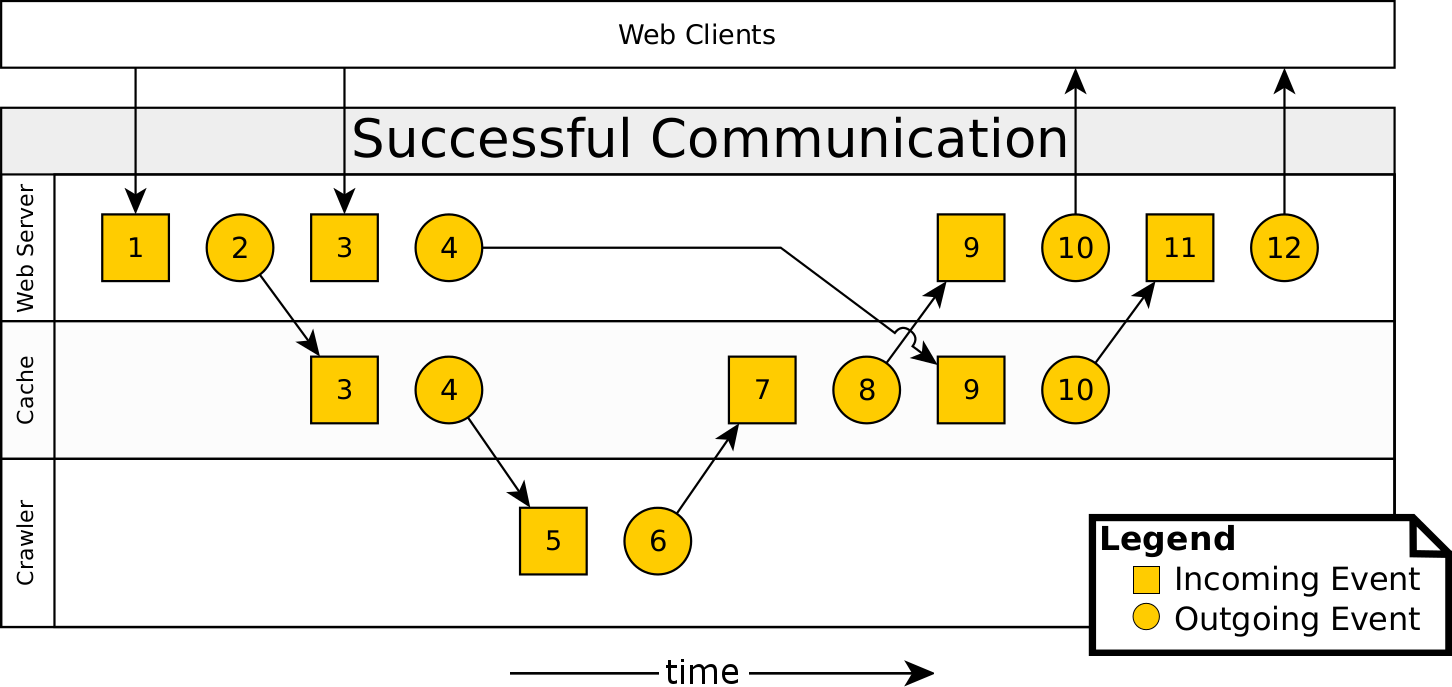
\includegraphics[width=0.8\linewidth]{diagrams/communication_v2.png}
  \caption{A communication schedule}
  \label{fig:comm-sched}
\end{figure}

To be useful for debugging, the logical schedules we record have to be
sufficiently detailed to capture differences across multiple
executions. Assuming that servers are otherwise deterministic, we have
to record order, direction, and communication partners for each
network event in a distributed application. This can be done with
little overhead both in space and time during the actual
execution. The necessary information overhead we have to encode into
each event consists of 8 byte Lamport clocks~\cite{Geels2006Replay},
with the first bit as a sign byte to tell incoming from outgoing
events. Additionally, we include \textsc{IP} addresses and port
numbers to identify the communication partners, which adds 4 bytes for
the port and 16 bytes for the address, in the worst case of
\textsc{IPv6} addressing. For an application that keeps the last
1,000,000 requests stored in its logs, this amounts only to about 26
MiB in additional storage space. The additional time required to
encode this information is negligible, inducing a slowdown of only 1\%
in our \toolname, with most of the time spent waiting for network \io
operations.

\begin{table}[h]
  \centering
  \begin{tabular}{l | c c}
    Benchmark & Avg Executions/5s & $\sigma$ \\
    \hline
    Normal execution & 8.51 & 0.31 \\
    Recording & 8.39 & 0.12 \\
  \end{tabular}
  \caption{Executions of a script that exercises the described flight
    booking bug. We ran the script 50s and averaged the number of
    executions per 5s}
  \label{tab:tracing-bench}
\end{table}

Figure~\ref{fig:architecture_1} shows how the different modules
collaborate during recording. The Path Tools suite runs test cases, so
the developer writes a test case that (``sometimes'') reproduces the
bug. We call this test case a \emph{diagnosis script}. This script
creates \ac{http} traffic. The \lstinline{HTTPSocket} class is
responsible for sending this traffic to the network. We have created a
Context/S layer for recording that layers the \lstinline{HTTPSocket}
class and records a process-local trace of the network communication,
before passing the traffic on.

Network traces in \toolname include an integer id as Lamport clock,
the first 500 bytes of the message, as well as \textsc{IP} address,
\textsc{url}, and port for both sender and receiver for all sent and
received \ac{http} requests. These are saved in a process-local
structure and are not sent on the network. The recording layer also
adds the current Lamport clock ``time'' as an application defined
\ac{http} header to each outgoing request, and reads it from incoming
requests. This is \ac{http} specific, and for protocols that do not
have room for custom data, a more general approach---such as
prepending magic bytes to the payload---can be
used~\cite{Konuru2000}.

\begin{figure}
  \centering
  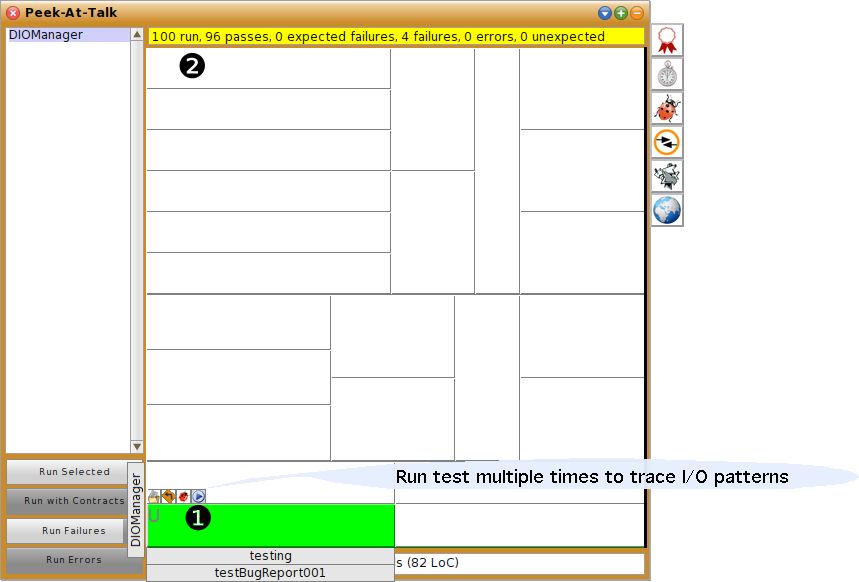
\includegraphics[width=0.7\textwidth]{screenshots/recording.png}
  \caption{\toolname integration in PathMap tool}
  \label{fig:pathmap}
\end{figure}

Activation of the recording layer is completely transparent to the
users of \toolname. When they run a test case as a diagnosis script
through the PathMap tool (\cf{\autoref{fig:pathmap}\textcircled{\small
    1}}), \toolname asks how often the script should be executed (this
number has to be chosen from experience, finding a number of
executions that shows around a dozen failures seems to work well -- so
for a script that fails 10\% of the time, 100 runs are ok.)

After each recording, \toolname merges the traces from different
processes into a list, sort events by id, and assigns the result of
the test case to the trace. This way, each trace consists of a list of
events that include communication partners and a Lamport clock, as
well as a test result. Test results are gathered and shown in a banner
in the \ac{ui} (\autoref{fig:pathmap}\textcircled{\small 2}.)

\paragraph{Schedule Shaper}
\label{sec:traffic-shaper}

The first goal of record and refinement is to enable consistent
reproduction of failures in the live system by removing the network as
a source of non-determinism. From the data recorded during multiple
executions, we constrain the system to those communication schedules
that exhibit the failure. For this we use a \emph{traffic
  shaper}~\cite{IetfShaper}, which, for each node, controls the
interaction with \io devices and mediates application access to the
network.

The scheduler has to control all network access by applications. We
achieve this control by wrapping the runtime's network \ac{api}. All
data sent or received through that \ac{api} is treated according to
the recorded schedules. For this, the scheduler buffers each
event. Once all events that are expected to occur before a buffered
event have appeared according to the schedule, the buffered event is
released. In the case of a single-threaded server, any interaction
with the network is served from the buffer if possible, and only
executes the wrapped functions if no suitable event is available. The
scheduler will keep executing the wrapped function and add the result
to its buffer until a suitable event is available. On a multi-threaded
server, events are held back using semaphores that are signaled when
the previous event is released.

Our scheduler has to deal with situations in which no event occurs
that matches a required schedule. Such situations will cause an
application to wait for the network and appear to ``hang''. In cases
where a given schedule cannot be reproduced in the live system, for
example if a server that appears in the schedule has been taken
offline, we argue that developers have to be able to inspect the
scheduler operations to understand the situation. Appropriate
heuristics such as timeouts or conditions for giving up on a replay
attempt are developer configurable.

% constrain the communication in the system to failing communication
% schedules
% tame non-determinism -> make sporadic failure deterministic
% shaper: Intermediate layer b/w framework and runtime/system
% Buffers events until the right event is found
% releases events in order, as many as are available
% forces multi-threaded server into buffer by use of semaphores
% heuristics and additional info for developers (timeouts, unscheduled
% events, current buffer status)

\subsection{Anomaly Detection}
\label{sec:anomaly-detection}

To determine whether network races are the culprit of a failure, we
require developers to write a \emph{diagnosis script}. Such a script
is similar to a test case:
\begin{lstlisting}[%
  basicstyle=\scriptsize,%
  emph={testBugReport001},%
  emphstyle=\bfseries,%
  showstringspaces=false,%
  frame=tb,%
  columns=flexible]
  testBugReport001
    | priceTable flightIdIdx flightId price reservation |
    priceTable  := (HTTPSocket
                    httpGetDocument: 'http://localhost:4567/search'
                    args: {'origin' -> {'Berlin'}.
                           'destination' -> {'Amsterdam'}.
                           'date' -> {Date today printString}}) content.
    price       := (table
                    copyFrom: (table indexOfSubCollection: '<td>' startingAt: priceEndIdx - 9)
                    to: (table indexOfSubCollection: ' EUR')) asInteger.
    flightIdIdx := table content indexOfSubCollection: 'data-id="'.
    flightId    := (table content copyFrom: idIdx to: idIdx + 20) asInteger.
    reservation := (HTTPSocket
                    httpPostDocument: 'http://localhost:4567/flights/', id, '/reserve'
                    args: nil) content
    self assert: (reservation endsWith: price asString).
\end{lstlisting}

In our example, the script mimics the behavior of a customer who
reserves a seat on an airplane. It communicates with the Web server
via \ac{http}, and asserts that the returned data has the correct
rates. We use assertions to classify recorded network communication
schedules in relation to whether they produce a failure. Variances
between successful and failing communication schedules can be used to
reduce the number of network events that developers need to consider
during debugging.

For our anomaly detection, we repeatedly apply the
\ac{lcs}~\cite{Bischof2008AiA} differencing algorithm to groups of
communication schedules. First, we determine \acp{lcs} of all
successes and all failures respectively, removing outliers. Second, we
diff \acp{lcs} of successful communications with \acp{lcs} of failing
communications. The differences between those are most likely to
contribute to a failure. In Figure~\ref{fig:comm-comparison}, we have
only one successful run at the top and one failing run at the bottom
left, so the \acp{lcs} of failures and successes are trivially to the
full communication schedules each. We compare those and find the
differences between successes and failures in the shaded and magnified
area.

For more complex examples, anomaly detection requires more recorded
executions to detect anomalies. Assuming otherwise deterministic
servers, successful schedules will exhibit fewer anomalies and thus a
sufficiently large number of failing and successful executions will
ensure that the anomaly detection can exclude variances that have
little or no impact on the failure.
% This needs some validiation and explanation

% If the servers exhibit other non-determinism, additional detection
% of such is required to discards unsuitable executions, \eg if a load
% balancer is present, the test script has to fail if a different
% server is used

\begin{figure}
  \centering
  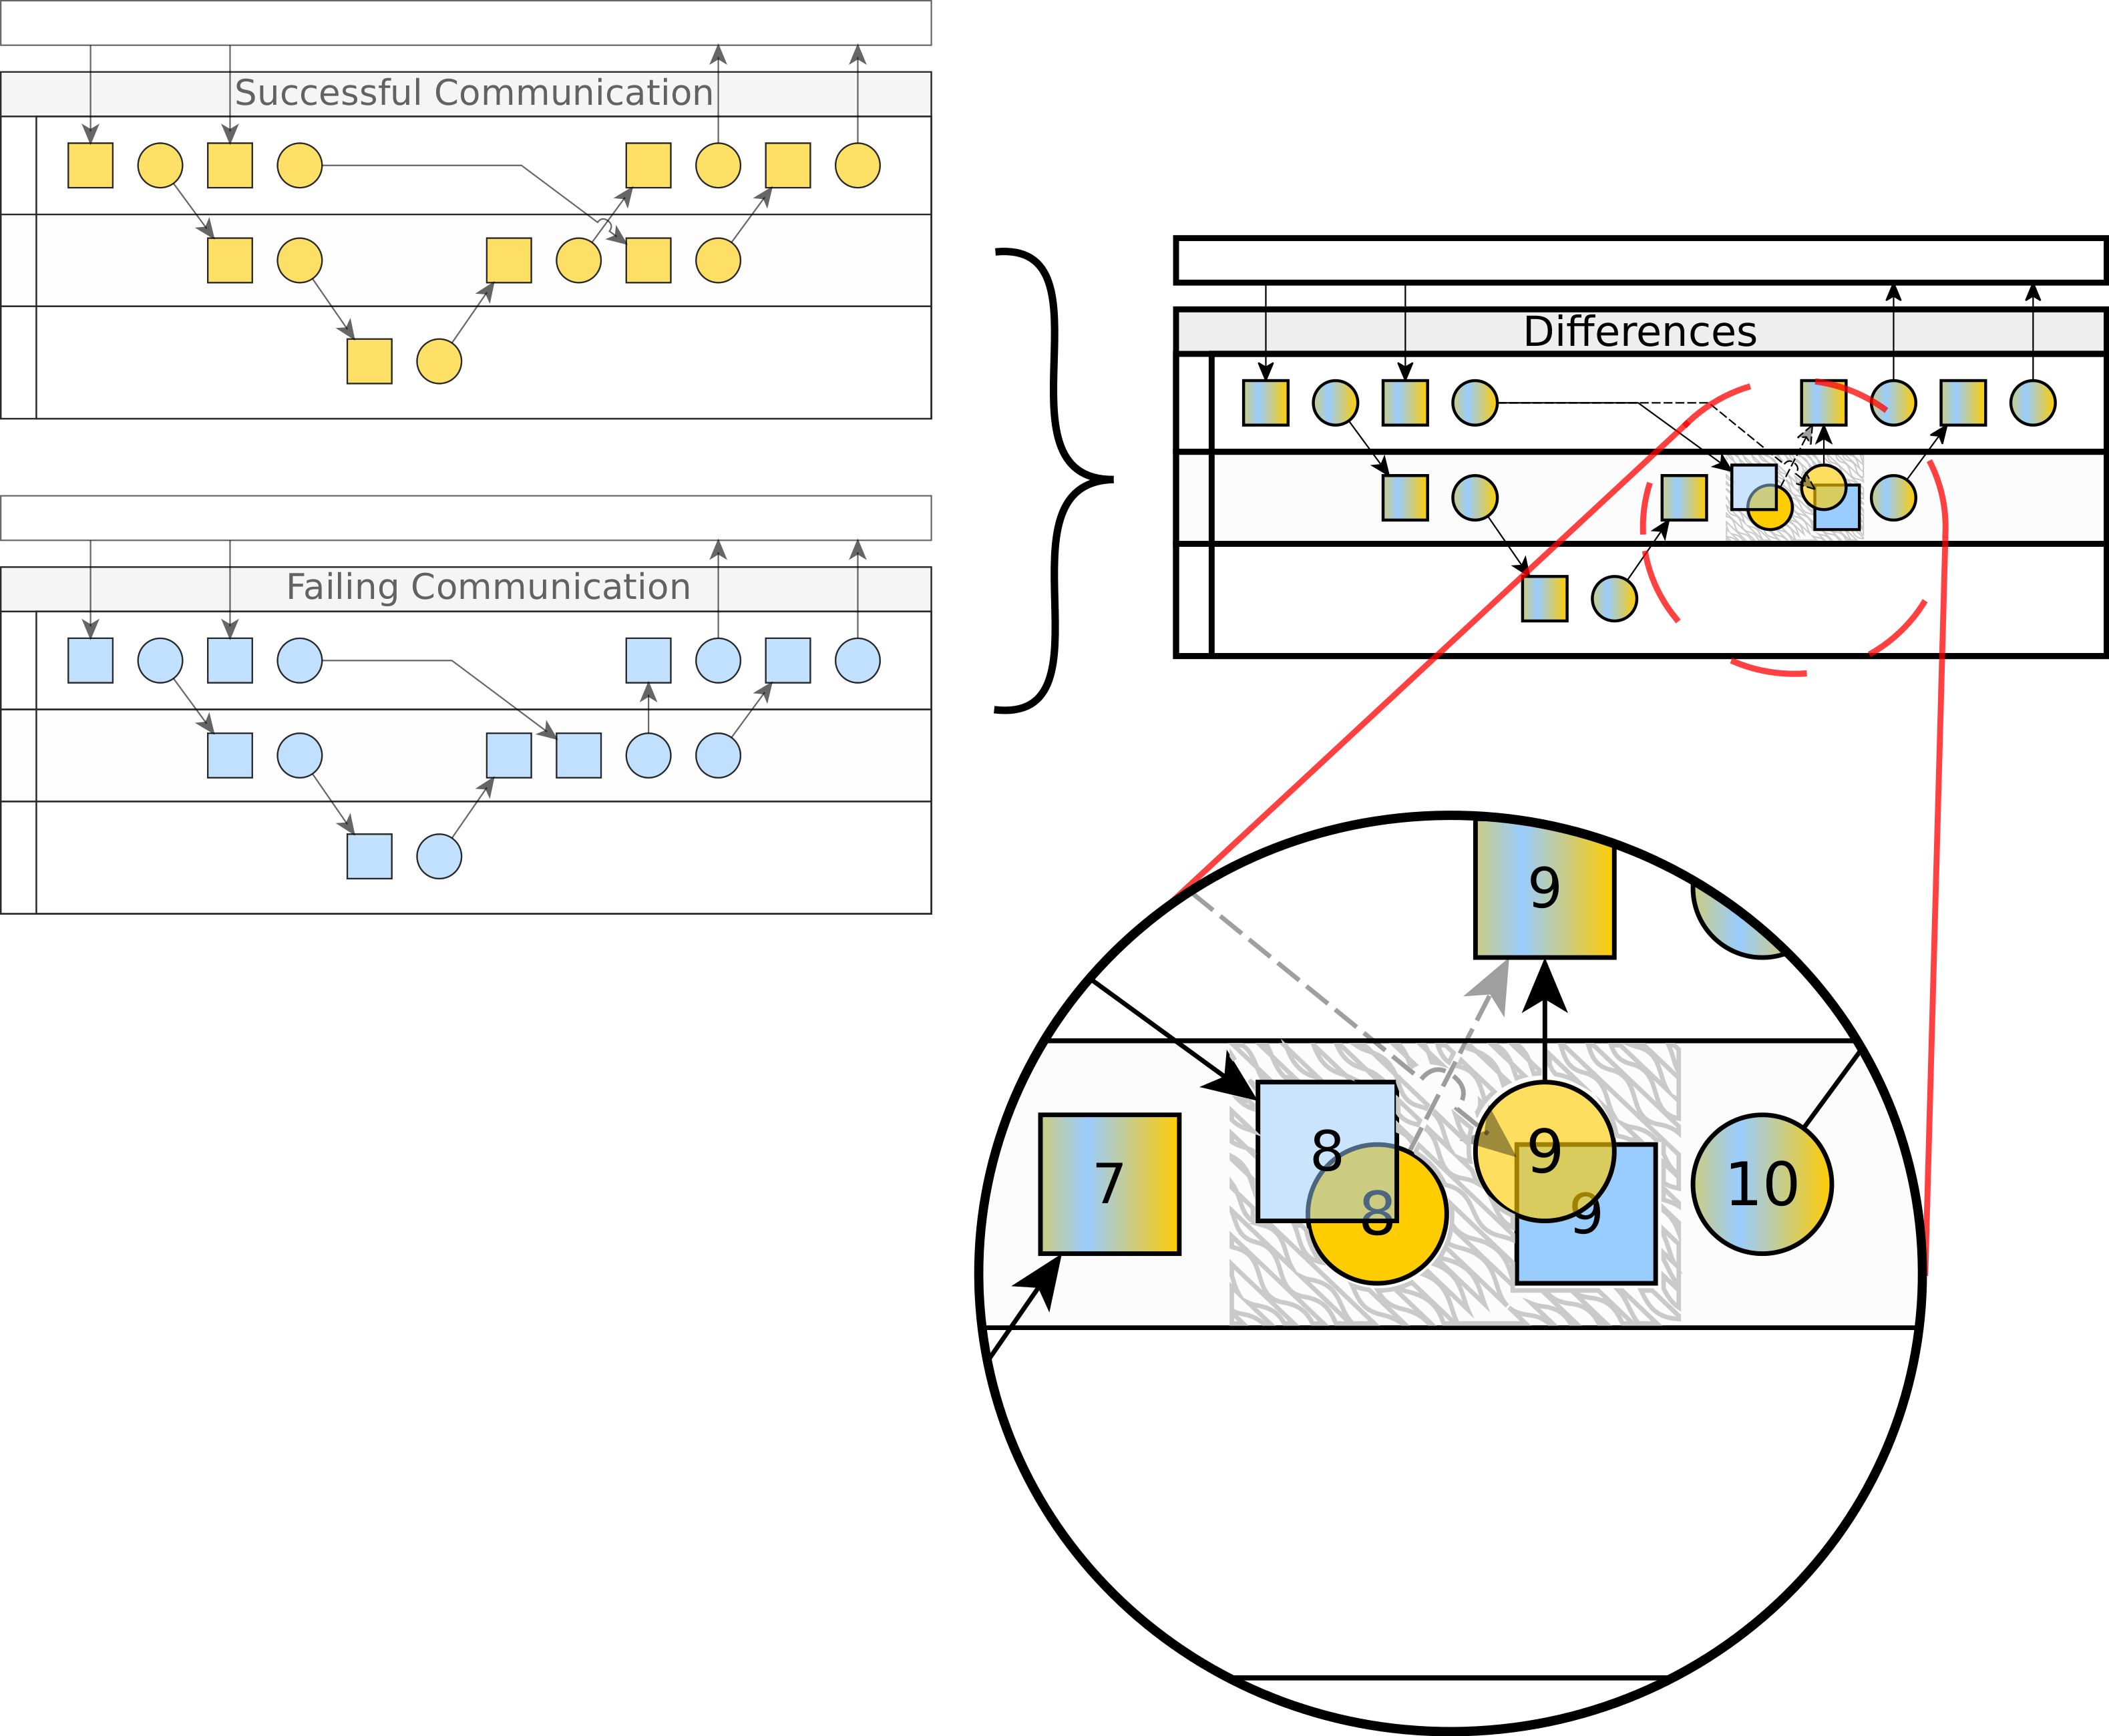
\includegraphics[width=0.7\linewidth]{diagrams/diff_v3.png}
  \caption{Anomaly detection for two schedules}
  \label{fig:comm-comparison}
\end{figure}

% assume failures are caused by non-determinism in communication schedule
% use reproduction in live system for recording
% what to record?
% ordering of events is paramount -> human reasoning
% assume servers are deterministic in themselves -> communication schedule suffices for replay
% record lamport schedule (reference to previous work)
% end up with communication schedules that lead to failures (more
% often -> statistically?)

\subsection{Refinement of Remote Data}
\label{sec:data-refinement}

If communication timing dependencies are the source of a
non\-/deterministic failure, then the system will fail consistently
when constrained to failing communication schedules. Once developers
reviewed and understood the high-level dependencies, they need to
understand how they are expressed at the source code level to fix the
failure.

Using our scheduler, developers can inspect specific failing
communication schedules for further analysis. The scheduler provides
an interface to add queries to events.  The first time a developer
re-runs a schedule, \toolname adds a query to record the stack at the
time each event is released. When this schedule is applied to the live
system, our scheduler records which methods are active before each
event is released and returns that data to our debugging tool. A
developer can then select an event in the communication view, and the
debugging tool will present a partial call tree that corresponds to
the selected event (\cf{Section~\ref{sec:data-refinement}}).

Developers can explore the call tree and request additional
information about method arguments and return values, as well as
instance variables of objects. Based on the recorded stack, \toolname
displays the method source code, if it is available. If developers try
to inspect, for example, a method argument, our tool attaches a query
to the scheduler in the live system. The scheduler wraps the
corresponding method and creates deep copies of its arguments and
return values during the next re-execution, which are then returned to
the debugging tool\footnote{For copying objects, we rely on Smalltalk’s 
\texttt{veryDeepCopy} protocol, which relieves us of the burden of 
dealing with details of copying. If necessary, this protocol also allows 
developers to adapt the analyzed object depth to their needs.}. Developers 
can drill into object references
analogously.%  \todo{actually hook this up}

This approach is an extension of step-wise runtime
analysis~\cite{Perscheid2010}. Developers can follow the information
available in the live system until they understand the failure,
without causing a significant one-time overhead. The overhead of each
exploration step is small, because we only selectively record
information that developers request.

% \todo{}
% interactive analysis -> interactive debugging
% record additional info for inspections (debugger) -> variable values,
% stack, arguments
% during re-runs
% developer can choose
% use stack to associate code locations
% no stepping, debugging from network events to code

\subsection{Discussion}
\label{sec:discussion}

The presented approach currently has two main limitations. First, our
low-overhead recording and schedule shaper depend on the determinism
of each server. Consequently, if other sources of non-determinism,
such as system calls to \texttt{random} or \texttt{gettimeofday}, have
an impact on the failure, we cannot currently reproduce it. This can
be fixed by recording more sources of non-determinism, at the expense
of increased overhead. This can be easily implemented with additional
layered methods around such non-determinism. However, our scheduler
could still use that additional data to constrain the live system to
reliably reproduce a failure, and the rest of our approach still
applies.

Second, our approach currently only works in the \emph{closed-world}
case, in which all processes that participate in the distributed
system include our recording and scheduler. If that is not the case,
we need to extend our approach in two ways to support an
\emph{open-world} case: first, we need to use a discovery mechanism to
tell participating processes from non-participating processes. Second,
for non-participating processes, we need to record the message
contents besides what we currently record. If a schedule is later
applied to the live system, events from and to non-participating
systems are replayed from the recorded data. Note that this may not
work if data returned from non-participating servers is
time-dependent, in which case our approach is not applicable.

\begin{figure}
  \centering
  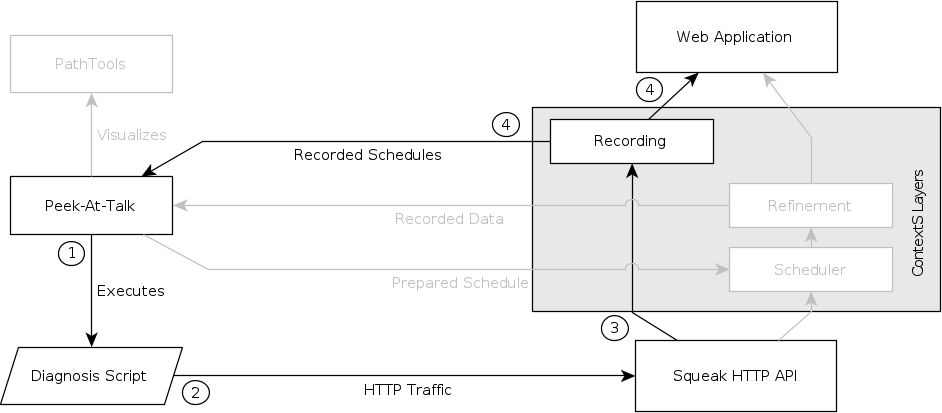
\includegraphics[width=0.8\linewidth]{diagrams/architecture_1}
  \caption{Communication Recording Phase}
  \label{fig:architecture_1}
\end{figure}

% \todo{}
% local reproduction?
% traffic shaper depends on determinism?
% discovery mechansim for open/closed world
% closed world -> all have scheduler and recording
% use dedicated interface
% open world:
% no scheduler => record message contents, (mock system)?, live system,
% oh no
% no recorder => easy to get bad schedule

\section{Implementation}
\label{sec:implementation}



\subsection{Anomaly Detection}
\todo{explain how we iterated over the algorithm -- short feedback
  loops}

For anomaly detection, \toolname requires developers to write a
diagnosis script which can be executed to gather communication
schedules. If the script includes assertions that check for the
presence of a failure, \toolname automatically compares and highlights
anomalies of the failures as shown in
Figure~\ref{fig:anomalies}. Developers can then begin their
investigation with these anomalous events.

\begin{figure*}
  \centering
  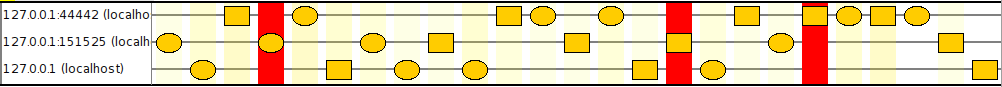
\includegraphics[width=\linewidth]{diagrams/prototype_diff.png}
  \caption{Highlighted anomalies}
  \label{fig:anomalies}
\end{figure*}

% \todo{Implementation genauer Beschreiben?}

% record: Squeak/Smalltalk, contextS, wrap framework methods, track
% sender/receiver/lamportId, some content -> implementable on other
% runtimes with other COP impls

\subsection{Refinement of Remote Data}

\begin{figure}
  \centering
  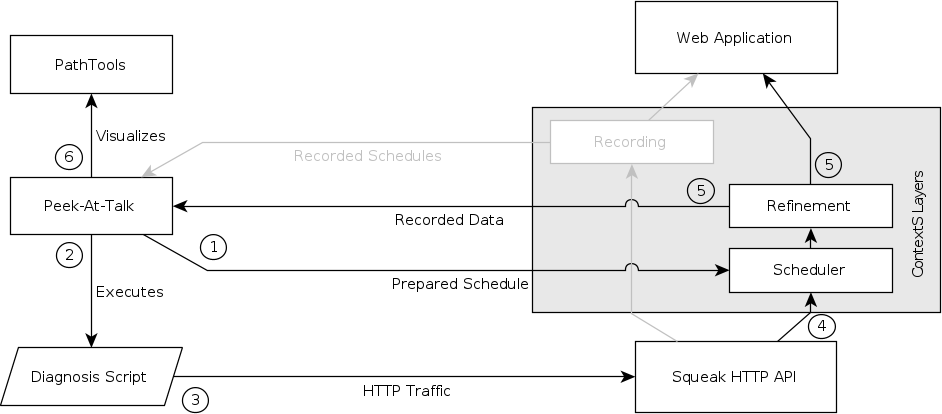
\includegraphics[width=0.8\linewidth]{diagrams/architecture_2}
  \caption{Scheduling and Refinement}
  \label{fig:architecture_2}
\end{figure}

The scheduler layer, when active, constrains the system to a
particular communication schedule. Figure~\ref{fig:architecture_2}
shows that the schedule is selected from \toolname, and then the
diagnosis script is re-run. The schedule layer keeps a thread-safe
input and output buffer to re-order network events as required. A
schedule contains a recorded trace with queries to the refinement
layer. Developers can inspect an event more closely by selecting it
graphically, and \toolname will activate the scheduler layers for each
process with the corresponding schedule and queries. The first time a
developer selects an event, a query is added to record method
invocations around it. The process that generates that event leverages
the reflective capabilities of Smalltalk to gather execution data and
return it to the \toolname debugger, which combines recorded method
invocations and visualizes them in a call tree. 

\begin{figure}
  \centering
  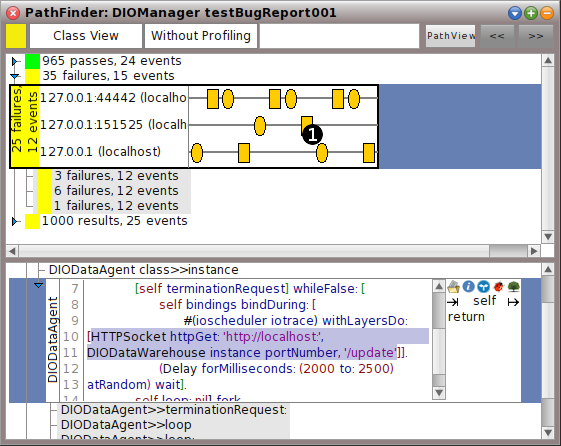
\includegraphics[width=0.8\linewidth]{diagrams/refinement.png}
  \caption{Refinement of an event in the network schedule (top) to
    show the corresponding application method (bottom)}
  \label{fig:refinement}
\end{figure}

In Figure~\ref{fig:refinement} we show the result of a developer clicking
event \textcircled{\small 1}. If the source code for the displayed
methods is available in the image running the debugger, the
application method closest to the event automatically
opens. Developers can then select method arguments or receiver
instance variables for inspection, which causes other queries to
execute.
\todo{screenshot title includes PathFinder - replace with \toolname?}

%\begin{figure}
%  \centering
%  \includegraphics[width=0.8\textwidth]{diagrams/ImplementationOverview}
%  \caption{The Path Tools framework is integrated into the Squeak/Smalltalk development environment and consists of a dynamic analysis framework and the Path tool suite}
%  \label{fig:pathToolsArchitecture}
%\end{figure}


\todo{maybe compare to eclipse debugger extensions we did in orchideo??}


% shaper: contextS, process-global schedule, heuristics preferences
% (timeouts, drop or delay unscheduled messages), schedule is either
% active or not, schedule items each include sender/receiver/some
% content

% data refinement: schedule items include an optional query (only
% hardwired queries) -> keep stack, keep method arguments ... (uses
% smalltalk reflection, not sure how to implement in java)

% \section{Evaluation}
% \label{sec:evaluation}

% In this section, we evaluate our prototype in terms of performance and
% with a case-study.

% \paragraph{Performance}
% \label{sec:accuracy-performance}

% Our prototype uses ContextS to implement the tracing. We benchmarked
% executions of a diagnosis script that exercises the bug we described
% for our example flight booking service. We ran the script 10 times for
% 5 seconds each both by itself and with the recording layer active. We
% recorded how many times per second the script executes and averaged
% those numbers over the runs.

% \begin{table}[h]
%   \centering
%   \begin{tabular}{l | c c}
%     Benchmark & Avg Executions/s & $\sigma$ in \% of avg \\
%     \hline
%     Normal execution & 8.51 & 3.64 \\
%     Tracing & 8.39 & 1.36 \\
%   \end{tabular}
%   % \caption{Tracing Benchmark}
%   \label{tab:tracing-bench}
% \end{table}

% Our results indicate that the practical tracing overhead is minimal,
% inducing a slowdown of only 0.01. Although ContextS has a very
% high-overhead and is one of the slowest available implementations of
% \ac{cop}~\cite{Appeltauer2009} for send-heavy benchmarks, in the case
% of distributed applications, a lot of the time is spent waiting for \io
% and not in method activation. Given these results, a context-oriented
% implementation for other languages should equally have a very small
% practical overhead and thus fulfill the requirement for low-overhead
% tracing.

% % logging overhead of ContextS solution -> minimal, implemented on other
% % platforms, applicable

% \paragraph{Case Study}
% \label{sec:case-study}

% To evaluate our approach, we have re-implemented a system from an
% industry partner that exhibited a timing\-/dependent failure. The
% original system is written in Ruby on Rails and deployed in the
% intranet of a company with about a hundred users. The system
% implements a reporting Web service, which its users query to get
% current data about other systems within the company. A user will
% generally have a few prepared reports that provide a high-level
% overview about different sub-systems. If any of the overview reports
% are not within expectations, the user will drill into those reports to
% see more detailed listings of the available data.

% After this system was deployed, the developers received a bug report
% in which a user noted that very rarely the sums in the overview will
% not match the numbers returned when drilling down into the data. This
% rare bug was triggered if, between requesting an overview and a drill
% down, new data became available in any of the sub-systems and the
% drill-down query was run against the new data.

% We have reimplemented the system in Smalltalk, keeping the setup of
% servers and their responsibilities and communication the same as in
% the original, for evaluation with our prototype. Our participants did
% not know the code for the system beforehand, but we explained the
% purpose and setup before the trial. We provided the original bug
% report and explained we had already transformed it into a diagnosis
% script. Using our tool, the participants were able to understand how
% the participating servers communicate. Our anomaly visualization
% required some explanation, but then the participants could also
% identify the timing\-/dependency, as well as explain the problem in the
% source code associated with the anomalous events.

% % industry example of such a failure
% % re-implementation of setup in Smalltalk, debugging with our tools

\section{Related Work}
\label{sec:related-work}

Our approach builds on previous work in the area of distributed
post-mortem debugging and distributed record and replay. Current
approaches vary mainly in how much they record, and subsequently, how
much of the system they can simulate to eliminate behavioral
disturbance.

We draw ideas for our debugging tool and refinements approach from
Friday~\cite{Geels}, a debugger for distributed record and replay, and
Causeway~\cite{Stanley2009}, a distributed post-mortem
debugger. Friday provides extensions to the GDB debugger and enables
developers to add watchpoints and queries to a replay to gather more
information. Causeway synchronizes a network view with a call-tree, so
developers can easily map executed code to network events. In contrast
to these approaches, our record and refinement enables developers to
continuously use it on the live system to debug failures that occur
very rarely or never in development.

Our recording technique is similar to the record and replay as
presented in liblog~\cite{Geels2006Replay}, DejaVu~\cite{Konuru2000},
RecPlay~\cite{Gent1999}, and Jockey~\cite{Saito2005}, all of which
also use Lamport clocks and intercept \io to establish partial
ordering of network events. However, these approaches focus on
low-level network events and intercept \io at the level of systems
calls. They also require either a custom \ac{vm} or additional dynamic
libraries that cannot be deactivated at runtime. The low-level events
recorded by these approaches are further removed from the application,
which makes it difficult for developers to understand where they
originate in their application code. As the kind of data that is
recorded by these approaches is predetermined, developers cannot
easily test whether a given non\-/deterministic failure originates
from timing dependencies in network access. Compared to these
approaches, record and refinement is more flexible in what it records,
and does so at a higher level abstraction.

R2~\cite{guo2008r2} is an application-level record-and-replay approach
which offers more control to the developers about what is recorded,
and can be used to test for multiple sources of non\-/deterministic
failures. However, unlike our approach, R2 does not allow replay in
the live system.

Our record and refinement can be seen as an extension of dynamic
memory access race\-/detection in parallel programs such as
RaceTrack~\cite{yu2005racetrack}. Compared to such approaches our
implementation is less general. However, its advantage is the higher
level of abstraction, which is closer to the mental model of the Web
application developer. We argue that tools that detect a large set of
data\-/races, but do so by acting at a low level of abstraction, such
as memory regions and \io devices, are less useful in debugging
specific kinds of races than specialized tools such as \toolname.

% record and replay (DejaVu, liblog, iDNA, ReCrash)
% post-mortem (Causeway, \todo{more})

\section{Conclusions}
\label{sec:conclusions}

We have presented our \emph{record and refinement} approach to debug
non\-/deterministic failures in the timing\-/dependent communication of 
distributed applications. Our approach provides a
systematic top-down method to low-overhead recording of network events
in the live system, anomaly analysis, and refining of runtime data
from the live system. To evaluate our approach, we present our \toolname 
tool for debugging distributed Web applications.

Since the overhead of our recording approach is low, it can be enabled
in a deployed system continuously and record data about failures that
occur infrequently or only during deployment. We achieve this low
overhead by focusing on the data strictly necessary for failures
caused by timing\-/dependent communication.

Our anomaly analysis of communication schedules identifies network
patterns that are likely to contribute to a failure. Developers use
these associations to acquire an overview of the timing dependencies
in the system at a high level of abstraction and subsequently to
choose schedules and events for further inspection. We detect
anomalies by differentiating communication schedules and correlating
the differences with failed assertions.

Finally, we provide a refinement mechanism to selectively inspect 
runtime data in the live system. This allows developers to debug the 
failure at the source code level, without being restricted by the amount of
prerecorded information. We achieve this by constraining the system to
a particular communication schedule and wrapping method executions to
record runtime data.

Future work is two-fold. First, recording and scheduling should be
extended to other sources of non-determinism, to show that our
approach is applicable not only to timing\-/dependent
communication. Second, we are investigating how to integrate
non-participating servers into our approach. Furthermore, beyond
debugging of timing\-/dependent communication, we may investigate how
\toolname allows developers to gain an overview of a distributed
system. By connecting code locations on different servers via network
events it emphasizes the implicit programming interfaces between
servers and helps developers to understand how communication is 
performed in the code.

Despite these future work, our approach is already usable to debug
failures in distributed systems. We have evaluated in a case study how
developers can approach failures without prior knowledge of the
concrete distributed system. Our approach does not require the system
to stop, it allows debugging on the live system, and it allows
navigation on both network and implementation level.

% Future work:
% limitations of scheduler, open/closed world, local reproduction
% My conclusions:

% \chapter{Introduction}
\label{cha:introduction}

From its beginnings in the 1990s, the Web has become an important
application platform in less than one and a half decades. Industry
surveys indicate that an increasing number of companies develop
distributed Web applications as a core part of their
business~\cite{kondo2009cost,EYPaaSSurvey2012}. However, many of those
applications are not written with distributed systems middleware to
handle communication between services. Instead, developers improvise
their own communication interfaces. This is error-prone and
complicates integration~\cite{Nadiminti}.

Distributed applications are especially prone to software
failures. Recent studies~\cite{Ballou2008,Tassey2002} show a relative
increase in code problems, hidden dependencies, and accidental
complexity when integrating multiple systems. Different systems may
provide different network interfaces and developers need to understand
their utilization and implicit assumptions. Different systems also run
different frameworks and programming languages, so that developers
need help to associate observed network communication with code
locations. This additional complexity makes it harder for developers
to reason about the system as a whole, thus, they are more likely to
introduce defects~\cite{zeller2009programs}. Debugging the resulting
failures is hard, and we have identified four primary problems that
developers face with current approaches and tools.

First, reliably reproducing failures is hard. Since distributed
systems execute in parallel, a global event order is difficult to
establish and may vary non-deterministically across
executions~\cite{lamport1978time}. Such variance depends on the
physical connections between the servers. The development setup will
differ from deployment and, thus, network delays and probabilities for
non-deterministic behavior also differ. Consequently, developers may
not be able to trigger some failures during development that occur in
deployment, or such failures may occur so rarely that it is impossible
to debug them effectively, because developers cannot reliably
reproduce them.

Second, developers cannot easily distinguish between causes and
effects. Many developers rely on systematic logging to understand
failures that only occur during
deployment~\cite{zeller2009programs}. However, isolated event logs are
poorly suited to create a global view on the events in a distributed
application. The ability to reason about global event order is
necessary for humans to understand causality in a
system~\cite{lamport1978time}. Understanding the cause of a failure is
essential for fixing it correctly.

% Consider a search engine. For a small scale engine, developers can
% control data storage, transactions, and database connections. On the
% Internet, the primary communication protocol is \ac{http} which limits
% in the amount of control developers have over their systems'
% connections. Non-atomic data updates usually cannot be wrapped in
% transactions. Storage services on the Web cannot provide transactions
% to thousands of users in parallel. Parallel \ac{http} request are each
% stateless and provide no guaranteed ordering. Thus, developers can
% rely less on the underlying infrastructure and require debugging tools
% work in a distributed setting.

Third, developers cannot easily inspect execution on servers in the
system. With symbolic debuggers, programmers inspect execution state
and behavior to find anomalies that may have caused a
failure. Symbolic debuggers enable them to stop execution and
interactively inspect the program's state. However, in a distributed
system, developers need to inspect state across multiple servers,
which execute in parallel. Symbolic debuggers are tailored towards
systems under developer control, but not all parts of a distributed
system provide that kind of control. Stopping servers with a debugger
to inspect the execution state is not feasible during deployment and
external services may not provide any debugging mechanism.

Finally, different frameworks and programming languages on several
servers force developers to apply multiple debugging
tools. Consequently, developers cannot debug and inspect the
distributed system as one. Instead, they have to treat each system
separately, because current debugging tools cannot connect and
synchronize with others. Support for debuggers that work across
multiple servers and languages is virtually non existent.

Due to these problems, debugging failures in distributed systems,
especially non-deterministic failures, is a time-consuming task. It
usually consists of aggregating various forms of log files, debug
output, and \ac{api} documentation for the employed services, and then
debugging on an equivalent, local system to infer possible
problems. Symbolic debuggers cannot be used in distributed
applications, because they only support independent analysis of
individual processes and require full control over those.

Tool support for network observation, log aggregation and debugging
across different systems is virtually non-existent. Yet, to improve
programmer productivity, providing adequate debugging tools is a key
ingredient, as without them, debugging is a manual, time-consuming
task~\cite{Dinning1990}.

We argue that there is a need for debugging tools that target
distributed, heterogeneous systems which are not entirely under
developer control. Architectural patterns for the these kinds of
systems, such as \ac{soa} and \ac{rest}; and hosting services, such as
\ac{paas} and \ac{iaas}, are relatively new phenomena---the first
comprehensive description of \ac{soa} was in 2005~\cite{Erl2005}. For
that reason, much of the work in this area is still not aimed at the
specific challenges of debugging distributed applications. Developers
of these systems need tools that provide a means to record and replay
events consistently across multiple servers. The tools should
furthermore guide developers towards anomalous differences across
multiple executions, so developers can reason about causality in the
system. Finally, such a tool should allow developers to cope with
multiple frameworks and languages, as they are common in distributed
applications.

\section{Approach}
\label{sec:approach}

In this work we present an approach for integrated debugging in
distributed applications, targeted specifically at Web development,
but extensible to other kinds of applications with similar
problems. Our approach---Replay-driven Fault Navigation---combines
state of the art techniques in the area of record and replay to
eliminate of non-determinism, distributed program comprehension, and
statistical debugging.

To allow debugging of non-deterministic failures, we present a tracing
approach for unified monitoring of systems. We continuously monitor
the live system and record enough data to allow reproducing relevant
program state at a later time. Our monitoring imposes little overhead
so it does not disturb execution unduly and can stay enabled during
deployment. We analyze the recorded data and correlate it to failures
to determine causes and effects. Network schedules are treated as
sequences of send and receive events between pairs of servers. Our
heuristics assign cause probabilities to sub-sequences of the recorded
network schedules, to guide developers during debugging. Developers
can replay such event sequences with our network scheduler and
iteratively refine recorded execution data for inspection. The
scheduler is an intermediate layer that controls how network events
pass between the application code and the framework. It blocks or
stalls events to change the order in which they pass in and out of the
application to match the recorded sequence. We correlate the network
data with source code and present both in a unified debugging tool, so
developers can debug at either level of abstraction and correlate
source code across servers and languages.

The advantages of our approach over traditional stop-the-world
symbolic debuggers are: the impact on the runtime behavior is kept at
a minimum, the technique can be applied to the live system,
eliminating the need for a test setup, and the debugging tools can
help developers to logically connect source code locations across
different servers.

To our knowledge, the presented approach is unique in that it
explicitly tries to support debugging across different languages and
system with one integrated approach. Work on understanding and
debugging distributed systems has been on-going for some
time~\cite{Parker1983} and the state of the art has solutions for each
part of Replay-driven Fault Navigation, but no integrated solution
exists that we are aware of.

\section{Outline}
\label{sec:outline}

This work is structured as follows: in \autoref{sec:requ-based-distr},
we discuss the problem domain on a small example. We highlight
challenges faced by developers when working with current debugging
techniques. In \autoref{cha:solution-design}, we present our four-step
approach to those challenges, and how that approach could work in
different languages and deployment scenarios. In
\autoref{cha:implementation}, we discuss an implementation of
Replay-driven Fault Navigation in Smalltalk. Finally in
\autoref{cha:evaluation}, we use the initial example and a larger
application adapted from an industrial system to evaluate our tool in
comparison with contemporary techniques. In
\autoref{cha:related-work}, we discuss related work and present our
conclusions in \autoref{cha:conclusion}.

%%% Local Variables: 
%%% mode: latex
%%% TeX-master: "thesis"
%%% End: 

% \chapter{Request-based Distributed Applications}
\label{sec:requ-based-distr}

A distributed application consists of a number of processes running on
one or more servers that are communicating over a network, for the
purposes of this work, the Internet. Such applications are especially
prone to software bugs~\cite{Ballou2008}. Software bugs are defects in
a program that developers introduce through an error in thinking. If
the defective code is executed it causes an infection of the execution
state. If this infection propagates to other states, it may eventually
become visible in form of a failure~\cite{zeller2009programs}. In this
work we focus on debugging distributed Web applications, but our
approach is applicable to other distributed applications as well.

Web applications are applications accessible through a Web browser,
with, at least, a client-side component for interaction and a
server-side component for data storage. Clients are written in
JavaScript to run in the browser, and the server components may use
any programming language. Many Web applications use \ac{http} as
transfer protocol, with event-loops to handle asynchronous
communication. The reason for this is the single-threaded nature of
JavaScript in modern browsers. In the absence of multiple threads or
processes, event loops are the only option to process multiple network
events in parallel on the client. However, developers increasingly
employ event loops for server implementations as well. Event loops
avoid spawning large numbers of threads or processes that are---due to
the potentially high network latencies across wide-area
network---waiting for IO most of the time. Web applications have at
least a client and a server component, but both often communicate with
other services. These, \emph{asynchronous request-based, distributed,
multi-language applications}, are the subset of applications this work
is aimed at.

The communication patterns of many distributed systems on the Web can
be described using \ac{uml} sequence
diagrams~\cite{rumbaugh2004unified}. In a sequence diagram, each
server is an entity with a lifeline for request handling, and receives
and sends asynchronous requests. Even though \ac{http} is a
synchronous protocol, if we regard both requests and responses as
asynchronous requests, we can treat servers that handle parallel
request using any mechanism as a single thread with only asynchronous
request-handling using event-loops.

\section{Motivating Example}
\label{sec:motivating-example}

We now present an example system that uses asynchronous communication
between multiple servers. Meta-crawlers are a type of Web search
engine that connect to other search engines. Meta-crawlers combine
information from other sources and provide a unified interface to
interact with that information. For example, flight booking systems
that offer multiple airlines connect to the systems of the different
airlines and provide a unified search and booking interface to
customers. Meta-crawlers such as these offer more than just search
across multiple providers, they provide additional services for
comparing prices, comparing seating options, or booking flights.

\subsection{System Description}
\label{sec:system-description}

We have built a system that implements such a meta-crawler and is
connected to a service providing fake airline data. It consists of a
Web site that allows the user to search for and reserve flights from
an origin to a destination on a specific date. The server serving the
Web site communicates with a cache. That cache provides flight
information and caches it for a certain amount of time. Such flight
information includes flight numbers, origin and destination of
flights, information about intermediate airports for a flight, as well
as pricing and available seats. This cache, in turn, connects to a
flight-data generator service that stands in for the airlines
providing information about their scheduled flights. All communication
is done via \ac{json}\footnote{JavaScript Object Notation\\
\url{http://www.ietf.org/rfc/rfc4627.txt}\\ accessed July 25,
2012}. The setup for this system is shown if
\autoref{fig:flyhehe-setup}, with the arrows indicating data
direction.

An intermediate query and cache service is an optimization that
meta-crawlers use, which avoids having to query the data sources
directly on each user request. Querying on each request is undesirable
due to network latencies and because data providers usually limit the
number of queries per time unit that meta-services can send to save
bandwidth and processing time. However, caches introduce the problems
of stale data and cache invalidation. Prices for seats on airplanes
usually rise as the flight date approaches, and as increasingly fewer
seats are available. Consequently, in order to create a reservation,
flight booking systems either cannot guarantee the exact prices for
their results, or they have to invalidate their caches and query for
current data at the time of reservation.

\begin{figure}
  \centering
  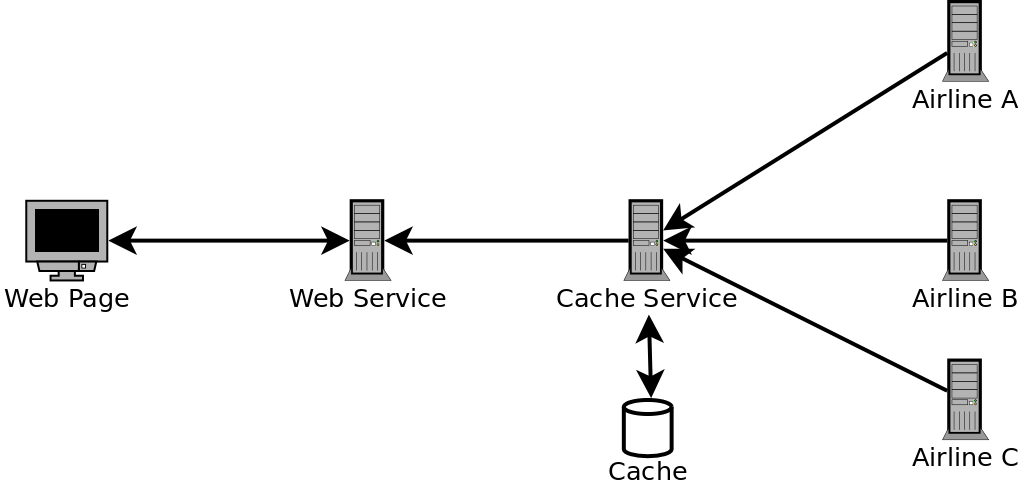
\includegraphics[width=0.7\linewidth]{flyhehe-setup}
  \caption{Flight Meta-Crawler Demo Setup}
  \label{fig:flyhehe-setup}
\end{figure}

\subsection{Failure Scenarios}
\label{sec:failure-scenarios}

Consider two customers on the meta-crawler Web page at the same
time. Both are looking for flights from Berlin to Amsterdam, as shown
in \autoref{fig:flyhehe}. The results of their search will be served
from the cache, and may not be the most recent data from the
respective airlines. If both customers try to reserve seats on flight
\emph{LH1009} at roughly the same time, different things may happen.

First, depending on the geographical location of both users with
respect to our system, the request for reservation may take some time
to reach the server. Depending on the time difference, one reservation
may complete entirely before the other request even arrives at the
server. As we have said above, in order to create a guaranteed
reservation, the Web server has to query the airline data---or, in our
case, the fake airline data generator---for the most recent rates and
available seats. Let us assume that the cache data was current and the
first reservation request can be fulfilled at the displayed rate of
156 EUR. By the time the second request for reservation arrives at the
Web server, the number of available seats has thus gone down to one,
which means the prices has gone up as the airline adjusts pricing
depending on available seats. Thus the second reservation can also
complete, but only at a higher rate.

Second, it may be that both requests for reservation \emph{arrive} at
our server at the same time, and are served in parallel. This leads to
a race condition for which we cannot deterministically decide which
one of the users receives the lower rate and which one the higher
rate. Either way, we, as the provider of the meta-service, do not want
to end up reserving two seats and receiving only the lower rate from
both customers, because in that case, depending on our and the
airlines' terms of service, we may have to pay the price difference or
a fine, which may not be a sustainable way to make business. At the
same time, as a customer, we do not want to create a binding
reservation at any other rate than the one shown on the Web site at
the time of our click on the \emph{Reserve Seat} link.

\begin{figure}
  \centering
  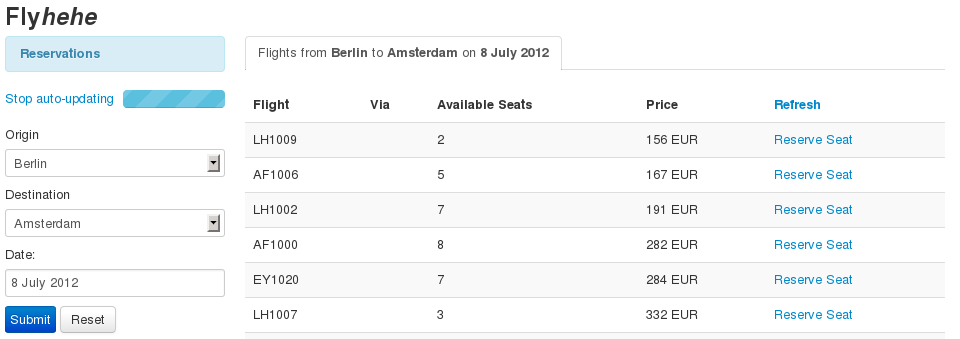
\includegraphics[width=\linewidth]{flyhehe}
  \caption{Flight Meta-Crawler Demo System}
  \label{fig:flyhehe}
\end{figure}

There are a number of challenges for the developers of such a
system. First, they have to understand the communication patterns that
may arise in production, with parallel access to the Web site, cache,
and airline data. They have to implement ways to deal with data races
and non-determinism caused by network delays. To do that, they have to
understand how non-determinism may lead to undesired states in their
application, such as making a wrong reservation. To verify their
solutions, they need a way to reliably reproduce problems and test
them. Finally, they need to understand how communication between two
systems tightly couples them at the implementation level, which means
they have to understand how changes to the code in one system may
impact that systems' ability to communicate with the others.

\subsection{From Bug Report to Failure}
\label{sec:from-bug-report}

A bug is an expression of a defect as a visible failure in the output
of a system. To fix a bug, developers have to understand the failure,
find the underlying defect, and remove it. Imagine the following bug
report for our flight booking system:

\begin{quote}
  Sometimes, when I try to book a flight on your website,
  it is added to my cart just fine, but with a different price than what
  it was in the list when I clicked it.
\end{quote}

This particular bug report is at a high abstraction level, as it
describes only user-facing input and effects. For such bug reports,
the first step towards fixing them is to reproduce them. Second,
developers should write a minimal piece of executable code that
reproduces the failure, so they can easily check their attempts at a
fix. Then the actual process of debugging can begin, which will
eventually make the test case pass.

These steps can be time-consuming, especially for very abstract bug
reports. Tools such as \emph{ReCrash}~\cite{Artzi} attempt to generate
test cases automatically, but can only do so for deterministic
failures. The above bug report contains the word "sometimes",
indicating a degree of non-determinism. That non-determinism may have
a number of causes. In this case, it may be that the user attempts to
book flights slightly differently without noticing. There may be
conditions in the environment, from browser bugs to transient hardware
failures, that cause the issue to only appear sporadically. Or there
may be non-determinism in the Web server implementation or the network
communication.

To approach non-determinism during debugging, developers have to check
each possible cause and try to eliminate it. Most of these causes,
including network communication, are difficult to reproduce faithfully
outside the live system. Unit tests are likely to be too low-level to
expose complex interactions, and acceptance tests running in a test
setup experience different conditions if the test setup is not
similar enough to the live system. Developers cannot with certainty
know whether a test setup sufficiently models the live system to
reproduce a given failure.

Given the above bug report and its possible causes, developers at some
point have to inspect the network communication schedule if no other
cause can be found.

\paragraph{Scripted Diagnoses}
\label{sec:scripted-clients}

Instead of acceptance or unit tests in controlled test environments,
developers may employ \emph{system diagnoses} as "test cases" to
simulate user input against the live system. Oftentimes those are
simple scripts simulating a browser's communication with the Web
page. This enables developers to include the circumstances under which
the bug occurred in the test. Even if the bug only occurs "sometimes",
repeated execution of the system diagnosis will eventually reproduce
it if it is related to varying network schedules.

This is the approach taken by tools such as
\emph{iDNA}~\cite{Bhansali2006} and statistical debugging
approaches. The deployed application is observed over long periods of
time, possibly through multiple occurrences of the failure. If the
failure occurs, as established by the bug report, "sometimes", then
the diagnosis is good enough for Replay-driven Fault Navigation.

\section{Challenges when Debugging in Distributed Environments}
\label{sec:debugg-distr-envir}

In distributed systems such as our flight booking system, developers
face a set of challenges in addition to the challenges of
non-distributed systems. The implementation of each service has to
account for the unreliable network, developers need to understand the
services they communicate with, and how data is represented and shared
between those
services.\\

\begin{description}
\item[Non-determinism] Non-determinism may have different causes: from
  randomness in the implementation, varying shared resource access
  order, to interactions with other processes and the operating system
  schedule and transient faults in hardware. Non-determinism here
  means that for equal inputs, the output and execution speed of a
  program is indeterminate.

  For a distributed system, non-determinism may mean that for an equal
  number and order of messages sent from one server, another server
  may produce different responses. A cause unique to distributed
  systems for this is network latency and request re-ordering. Sending
  a number of \ac{http} requests in one particular order does not
  guarantee its delivery in the same order. This is an instance of a
  leaky abstraction. \ac{http} messages may be broken up into multiple
  \ac{tcp} packets. \ac{tcp} packets may arrive out of order, and are
  collected by the operating system and delivered to applications in
  the original order for a connection. If the \ac{tcp} packets for one
  \ac{http} connection are available, the operating system passes
  those packets to the application, which handles them as \ac{http}
  request. The application does not know that another \ac{http}
  request is on its way that was sent earlier from the point of view
  of the sender. So, if the processing of any request is influenced by
  any other, network latency may introduce non-determinism.

  Network latency varies across network segments. Usually, during
  development, distributed systems are deployed in a test environment
  in an attempt to simulate the distribution properties of the
  deployed system. However, actual network latency during deployment
  is hard to predict, and data races across the network will only
  randomly be reproduced in a test environment. Furthermore, during
  development, \emph{click-races}---the situation when two or more
  users try access a resource simultaneously---can oftentimes not be
  adequately tested. Finally, deployed distributed systems, due to
  ongoing communication, very rarely enter a globally consistent
  state, so proving a system correct for its projected uptime is
  difficult~\cite{Geels2006Replay}. The only predictable way to enter
  consistent states is to shut down and restart the whole system
  regularly, which is not desirable for many systems.
\item[Heisenbugs] Failures that occur only during or change during
  debugging are called \emph{Heisenbugs}~\cite{Gray1986}. They happen
  because the debugging tool, through its observation process, changes
  the runtime behavior of the observed program. For non-deterministic
  failures, this means that introducing logging into the system may
  cause different failures to happen, or the original failure could
  happen much more or much less frequently, or not at all. This makes
  debugging non-deterministic failures harder, because the developer
  cannot be sure that the observed failure is the same as the original
  one.

  Distributed systems exhibit Heisenbugs more often, because network
  access order varies even from slight disturbances, such as the
  operating system scheduler or other processes in the system. Most
  debuggers incur significant overhead~\cite{Corliss2005}, which
  causes equally great disturbances to network access order, which in
  turn may cause Heisenbugs~\cite{Gait1985}.
\item[Languages] When systems run on different machines, or even only
  in different processes, and they communicate not via the language
  calling mechanisms, but rather through foreign-function interfaces,
  shared memory, or network communication, connecting call trees in
  one language to another is a non-trivial task.

  A developer has to find exit and entry points for \ac{ipc} in all
  communicating systems, and relate the input and output data, to
  connect events within one system to another. This task is made more
  difficult by abstractions from the input and output, for example,
  while the operating system will deliver \ac{tcp} packets in order to
  a language runtime, a Web framework will assemble \ac{http} messages
  before passing the data on to the application. If systems use
  different abstractions, one working on the transport layer and the
  other on the application layer, it is hard to determine the
  corresponding communication entry points.
\item[Data Representation] Different languages represent data
  differently. Consequently, different kinds of persistent data
  representation come natural to the language users. Different data
  representations have to be converted into each other, which
  introduces additional complexity and another source for
  bugs. Because the connection between the different systems and the
  data conversion is usually hidden behind libraries and frameworks,
  failures that are caused by incorrect data exchange are hard to
  debug, because developers have to understand multiple systems and
  how they transform the data.

  For example, a web-page will naturally display information to a user
  in a visual manner, using nested \textsc{HTML}-\textsc{DOM} elements
  to express the information content in a user-friendly way. The
  JavaScript code running in the browser will usually, at least
  intermittently, store information as JavaScript objects or in
  \ac{json}. \ac{json} may also be the format used in \ac{http}
  requests to transfer data between the client and the server. On the
  server, the data may again be transformed any number of times
  between different runtimes, backend servers, and databases.
\end{description}
~\\
These properties make debugging distributed systems a laborious
task. We have identified the following four debugging activities to be
especially problematic and in need of a solution.

\subsection{Observation and Logging}
\label{sec:observation-logging}

The need for observation and logging of program state changes has
clearly been recognized in both research and
industry~\cite{Saito2005,altekar2009odr,Stanley2009}. Most Web
frameworks include logging facilities, different log-levels, and
separate logs for access, input, output, erroneous and successful
events. There are full libraries\footnote{Airbrake: The error app 
  \url{https://airbrake.io/pages/home}\\
  accessed June 25, 2012} and frameworks\footnote{Apache log4j
  Logging Services
  \url{http://logging.apache.org/log4j/1.2/index.html}\\
  accessed June 25, 2012}
that provide comprehensive logging facilities to applications.

Distributed system are setup differently during development than at
deployment time. Simulation of distributed systems or parts thereof in
small-scale development deployments, as used at development time of
such systems, allows developers to evaluate system behavior in a
simple setting, relative to the deployment setup. In such development
setups, developers have full control over each server, and the power
to stop and inspect each process at practically any point in the
execution of the distributed system. Apart from such small-scale
setups, developers use full-scale test deployments to provide a more
realistic setting for stress testing critical aspects of the
system. Using setups of varying degree between fully local deployments
and full-scale test environments, developers can control the amount of
realism their code is exposed to.

However, once deployed, distributed systems will over time encounter
situations that could not have been anticipated by the developers,
state changes accumulate, the underlying network topology changes,
and, for successful services, system load and parallelism increases
beyond what could reasonably be
tested~\cite{Geels2006Replay}. Long-running applications may
experience non-deterministic, low-probability failures that develop
over time. Thus, logging data from the deployed system is
indispensable for testing and debugging failures that occur during
deployment.

If problems occur, most logging frameworks have settings on how to
react, by sending emails, checkpointing the running application,
stopping and saving a stack-dump of the program state,
etc. \emph{heartbeat} services regularly check accessibility of
services, existence of error artifacts, or output of logging
frameworks, to filter and notify developers when a problem occurs in
the deployed system.

Logging frameworks and error artifacts are useful for debugging, as
long as only a limited number of frameworks is used. As long as logs
are similar in format and level of abstraction, they can be related to
one another. However, although most frameworks that are used in the
context of networked applications offer logging capabilities, there is
no widely accepted standard for logging information and formats across
languages or frameworks.

\subsection{Understanding and Classifying Observations}
\label{sec:distr-reas}

Given appropriate logging, developers have to review and understand
the logs to determine how to approach a particular bug. This entails
associating parts of a log or particular log entries with
failures. Even for stack traces of single process applications, this
is no easy task, and developers can easily get confused about where to
look first in a trace~\cite{groetker2012Tdg}. For Web applications
developers have to understand and associate parts of logs from
different systems with the same failures. As different logs may expose
different aspects of the same problem, they have to be aligned with
respect to their order, so developers have chain of anomalous log
entries to follow backwards. Without such alignment, developers can
only guess which anomaly occurred first, and finding the cause of a
failure is a matter of trial and error. But aligning multiple logs is
a difficult task, unless there is a connected logging
facility. Minimal clock skew across systems may render timestamps
unusable for log ordering and parallel events cannot easily be
recognized as such.

Another problem presents itself when the failure is logged at a
different level of abstraction than the anomalies leading up to it.
For example, if the log entry with \ac{http} status code 500 on the
server represents the visible failure, the anomalies leading up to it
may be in form of database access or JavaScript exceptions, but there
may be multiple database accesses or exceptions for only one \ac{http}
request. Developers have to connect these anomalies and group them at
the right level of abstractions. Thus, understanding which log entries
are relevant to a particular failure is hard to determine as well.

\subsection{Reproducing Failures}
\label{sec:reproducing-failures}

Many debugging guides emphasize that the ability to reliably reproduce
a failure is crucial in the attempt to fix the underlying defect,
because it is the only way to make sure that an attempted fix is
successful~\cite{metzger2003Dbt,zeller2009programs,groetker2012Tdg}. This
can be difficult for single-process applications, however, distributed
applications exacerbate this problem. The \emph{global state} in a
distributed system is hardly ever consistent, unless the whole system
is restarted. That means that there is little opportunity for
checkpointing the system for running through a failure from the
checkpoint. To checkpoint a process, it needs to be in a consistent
state, so it can restarted later. For multiple processes, this means
that all nodes---and thus the complete distributed system---have to be
in a well-known state before a checkpoint.

Provided a consistent checkpoint can be established \emph{before} a
failure occurs, reproduction may still fail. Non-deterministic
failures caused by network latency or transient inconsistency in the
global state will not manifest each time the defective code is
triggered.

To deal with this problem, there are approaches to log \ac{http}
traffic on-demand, when a failure occurs~\cite{Konuru2000}. During
replay, instead of just running the complete, distributed system, only
one node is actually run, and interaction with external services is
replayed from records.

This is useful if the developer knows on which node the defect is most
likely to find. If that is unclear, however, the developer can only
replay and debug on each node, sequentially, until the defect is
found. For large numbers of communicating nodes, or if the error is
not on any node the developer can access, this is a time-consuming
process that may not lead to success.

\subsection{Connecting Server Events to Code Locations}
\label{sec:conn-serv-code}

Provided a useful log and a replay mechanism exist, and developers
have identified server events and servers that contribute to a
failure, they have to change the level abstraction from network
communication and servers to communicating processes and source code
to find and fix the defect. In distributed systems, it is not possible
to set a \emph{breakpoint} on a network event, and stop all services
that are communicating at the time to inspect them.

In order to deal with this problem, developers use logging in
different ways. Simple logging mechanisms or frameworks can be used to
determine the executed code around a particular network event. This
increased logging can be enabled on-demand, and log, for example,
method activations, arguments, and the data that is sent and received
over the network~\cite{Artzi}. Another approach is to save a full
continuation of the running program when a particular event
occurs~\cite{ducasse2010dynamic}. This continuation can later be
inspected with a symbolic debugger.

The problem with these approaches is that they only provide a
one-to-one connection between a network event and a code
location. Yet, code locations are connected across servers via the
network, so multiple code locations contribute to the same
request. Developers need to identify the same network events as they
are logged on different servers, to find those connections, and the
debugging tools have to provide this identification.

\subsubsection{Working with Multiple Call Trees}
\label{sec:work-with-mult}

Debugging across communicating processes is similar to debugging
across multiple threads. First, in both cases it is impossible to stop
all execution in one atomic step. Second, all processes and threads
have a separate stack as well. However, in contrast to multi-threaded
applications, distributed applications cannot communicate through
shared memory and have to use an \ac{ipc} mechanisms instead. In the
case of Web applications, \ac{http} \acp{api} are the \ac{ipc}
mechanism.

Consider again the sequence diagram for expressing the runtime
behavior of distributed systems. As per the \ac{uml} standard, nested
calls can be expressed using nested lifelines. Generally, that would
be the case if a method call from one object to another causes the
receiver to call another method on itself or a third object. For
distributed applications, this can describe the relation of network
messages and call trees. An \ac{http} request will trigger some code
to be executed on the receiver. While the level of abstraction is
different, in effect, this is equal to communicating threads and their
interleaved call trees.

Each node executes code in one language, on one or more threads. The
language runtime takes care of delivering calls to and return values
from call-sites. On the network, the \ac{http} layer has that
responsibility. This means, that in distributed systems there are
multiple, nested layers of \emph{runtimes}, each with their own call
mechanism.

Developers of multi-threaded programs need to be able to move between
call trees freely. The same applies for developers of distributed
systems. While thread call trees within one runtime are at the same
level of abstraction, network call trees and different language
runtimes are not. There is very little support for connecting those
layers within debugging tools, and methods for doing so are still
being researched~\cite{Stanley2009,Geels2006Replay}.

%%% Local Variables: 
%%% mode: latex
%%% TeX-master: "thesis"
%%% End: 

% \chapter{Replay-driven Fault Navigation}
\label{cha:solution-design}

With Replay-driven Fault Navigation, we address four challenges when
debugging distributed applications: observing and logging failures,
classifying and connecting logs, reproducing failures, and associating
server events with code locations. More specifically, our approach
consists of the following four steps:

\begin{enumerate}
\item We employ a lightweight record or logging mechanism on each
  server, to collect information about communication in the
  network. We combine the separate logs into one, by means of partial
  ordering using Lamport clocks~\cite{lamport1978time}. This step
  provides an improvement over the heterogeneous and unordered logs
  developers have to deal with today.
\item We identify failing and passing runs among logged events by
  connecting assertion failures in the execution with observed network
  traffic. We compare failures and passes to infer critical regions in
  the systems' communication patterns. Using this information,
  developers can focus on the relevant sections of the logs.
\item We use recorded communication as patterns to replay failing
  network schedules and check the replays for assertion failures. If
  the defect is related to a network scheduling problem, the failure
  will reproduce reliably. In that case, developers gain confidence
  that the failure is indeed caused by variance in the network
  communication schedules. Additionally, developers gain a means to
  reliably reproduce the failure for further debugging.
\item Finally, we use failure replay for debugging. We refine recorded
  data during replay to associate network events with code
  locations. We present both in a tool that allows developers to move
  between the two abstractions freely~\cite{Stanley2009}. This way,
  developers can inspect network events presumably corresponding to
  infected state at the program code level, an use additional replays
  to inspect execution state at this point.
\end{enumerate}

\section{Live System Observation}
\label{sec:lightweight-tracing}

In order to understand a bug, developers iterate over the same code
paths, inspecting different aspects of the program state. In order to
do so, they need some notion of logical event order, to infer causal
relations between events. In \autoref{sec:observation-logging}, we
also argued that it is important to have data from the live system to
debug distributed applications, because only the live system may
exhibit the specific timing behavior to produce a sporadic bug.

\subsection{Logical Communication Schedules}
\label{sec:logical-schedules}

Communication schedules in distributed systems can only be established
for subsets of all gathered network events, because communication
between servers in a distributed system is truly parallel, and some
events may thus happen at the same time, or so close in time as to
have no effect on one another. To understand causes and effects in a
distributed system, we have to establish the order of events in the
communication.

Network communication events occur at different levels of abstraction,
corresponding to layers of the \ac{osi}
model~\cite{zimmermann1980osi}. We chose to establish schedules at the
\emph{application layer} of the \ac{osi} stack, so they may be easily
correlated to the code that created them.  Previous work has mostly
focused on recording events on the \emph{transport layer},
i.e. \ac{tcp} and \ac{udp}
events~\cite{Geels2006Replay,Konuru2000}. However, network and Web
development frameworks usually work at the application layer, sending,
for example, \ac{http} requests or \textsc{sql} queries. These
high-level events may correspond to multiple events on the transport
layer. These transport events have little meaning for a developer
working on the application layer, but combining the transport events
back into application layer events is very difficult in a user space
library that does not have access to \eg \ac{tcp} sequence
numbers. Recoding schedules at the application layer allows us to
provide a user-space solution at a, for developers, meaningful level
of abstraction.

\subsubsection{Partial Ordering of Events}
\label{sec:lamport-clocks-1}

In most systems, the order in which events occur is fundamentally
important to our way of reasoning~\cite{lamport1978time}. We say that
event A happened at 3:15 if it happened \emph{after} our clock read
3:15 and \emph{before} it read 3:16. We call this order the
\emph{logical schedule}~\cite{Konuru2000} in which the events
occurred. The actual timing information (whether the event happened
\emph{at} 3:15, or between 1 and 59 seconds later), the \emph{physical
  schedule}, is only a more specific representation of that ordering.

However, for systems capable of parallel execution, such as the
distributed systems, a universal before relationship is not easily
obtainable and may not physically exist. To solve this problem,
logical, or \emph{Lamport} clocks~\cite{lamport1978time} are used to
establish a partial ordering. Lamport clocks provide a logical
schedule that can be implemented in a parallel system. Central to
logical schedules is the causality between events. If we know that an
event A triggered an event B, we know that A must have happened before
B, even in the absence of a clock.

The original implementation idea by Lamport, also implemented in this
work, is still widely
used~\cite{Konuru2000,Stanley2009,Geels2006Replay,altekar2009odr} and
extension such as Vector Clocks~\cite{Mattern1988}, Version
Vectors~\cite{Parker1983}, and Interval Tree Clocks~\cite{Paulo} exist
for more specific scenarios.

\subsection{Continuous Logging}
\label{sec:continuous-logging}

The traditional stop-the-world debugging approach is ill-suited for a
live system that only exhibits the erroneous behavior sporadically. We
have argued in \autoref{sec:conn-serv-code} that developers cannot
stop processes on different machines at the same time. First, this is
technically impossible, because there is no way to perfectly
synchronize all processes. Second, it is also impractical, as stopping
the live system will make it unavailable for users.

Other debugging approaches observe the live system and gather enough
data to allow inspection of the relevant program state at a later
time. One approach is to log all execution state~\cite{Stanley2009},
so developers can inspect that information offline at a later
time. However, such logging imposes a significant overhead, which
makes this approach unsuitable for continuous logging in the live
system. Other approaches~\cite{Konuru2000,Geels2006Replay} have shown
that it is possible to record just enough information to guide the
system down the right path during subsequent executions. These latter
approaches have little overhead and are suited for continuous logging.

We assume that each server in the network is in itself deterministic,
and that any non-determinism is introduced by access-races to shared
resources, i.e. the network and other servers. If each node is indeed
deterministic, that means that if network requests arrive in the same
order, the same \emph{class} of output---correct or incorrect---is
produced. Furthermore, we assume that nodes and the network are
well-behaved, meaning, that nodes do not suddenly change their
\textsc{IP} addresses, and network segments do not suddenly disappear,
making nodes unreachable. We realize that this may preclude usage of
our approach for less dependable networks.

This means we only have to record the order and type of \ac{http}
requests between any two communication partners to faithfully
reproduce communication, applying only traffic shaping. Compared to
recording the request contents or partial execution traces, this is
little information, with little space
overhead. Indeed,~\cite{Geels2006Replay} has shown that the necessary
information overhead encoded into the request packages may be as
little as adding an 8 byte Lamport clock. Since we do not store the
message contents, these 8 byte plus identifiers for the two
communication partners are all our storage requirements for network
events at runtime. As identifiers, \textsc{IP} addresses and port
numbers may suffice, adding 4 byte for the port and 16 byte for the
address, in the case of \textsc{IPv6} addressing. For an application
that keeps the last 1,000,000 requests stored in its logs before
rotation, this costs about 26 MiB in storage space.

Adding logging to an existing application will change its execution
behavior. The additional execution steps impact performance and thus
timing and memory behavior. Even slight changes can have a large
impact if they increase the likelihood of, for example, cache misses
in the \textsc{CPU}.

Nevertheless, choosing a lightweight logging mechanism is worthwhile
to minimize disturbance. Furthermore, by enabling the logging facility
in the deployed system, the overhead of logging is no longer a
sporadic disturbance that only occurs when running a system
diagnosis. Instead, the disturbed behavior becomes the normal
behavior.

Minimizing disturbance for debugging is particularly useful for
non-deterministic failures, but is a generally desirable property of
debuggers. It minimizes the potential for failures that occur only
during debugging, so-called \emph{Heisenbugs}.

\subsection{Mixed Environments}
\label{sec:mixed-environments}

With continuous logging in a distributed system one has to consider
organizational and practical boundaries. To introduce generalized
logging into a distributed system we need to extend services on
different nodes. Not all these nodes are under developer control, or
have source code readily available to extend them. Our tool thus has
to function in a mixed environment. For \ac{http} communication, this
is easily possible by adding custom headers, which will be ignored by
non-logging clients. We do not regard lower levels of
communication. Ways to deal with services at the transport level have
been covered in other work~\cite{Geels2006Replay,Konuru2000}.

Servers that are part of our distributed system, in the sense that
communication with them contributes to the purpose of the system, can
be either cooperating or non-cooperating. During normal execution,
non-cooperating servers simply ignore the additional headers for
Lamport clocks. To combine the logs at a later time, any discovery
mechanism, from a well-known port to ZeroConf\footnote{ZeroConf
  Internet Engineering Task Force (IETF) Internet Draft\\
  \url{http://www.watersprings.org/pub/id/draft-ietf-zeroconf-reqts-12.txt}\\
  accessed July 21, 2012} can be used.  Incoming and outgoing events
for sent and received requests, respectively, can then be added for
non-cooperating servers by means of inference.

This will necessarily create incomplete logs in the presence of
non-cooperating servers, but this can be safely ignored if no state is
shared with other, third-party, distributed systems accessing the same
non-cooperating servers. These systems are common in practice, because
\ac{rest} and \ac{soa} encourage cooperating systems without shared
state. However, this also means that our approach is not well suited
for shared, "cloud" database services and other stateful systems.

\section{Communication Analysis}
\label{sec:comm-constr-analys}

In Replay-driven Fault Navigation, recording communication events
provides data from the live system. Continuous logging will capture
correct and anomalous communication events. Developers need to
understand the difference, why one particular log ends with a failure,
where another ends without one. There is little tool support to find
such variances in server logs, consequently, this is the next step in
our approach.

\subsection{Differencing between Schedules}
\label{sec:diff-betw-call}

To create a tool to find variances in communication schedules, we need
a model of such schedules. We argued in \autoref{sec:requ-based-distr}
that sequence diagrams are well suited to both model network
communication as well message passing between objects. Consequently,
network schedules also form a \emph{call tree}, with requests and
responses representing message sends and returns.

However, network events occur at the higher abstraction level than
message exchange between objects, and differences to single-threaded
objects. In distributed systems, a single server serves more than one
request in parallel, using event loops or multi-threading to process
and send out responses as they become ready. Thus, we cannot assume a
causal relationship between two requests arriving at a server one
after another, and not between two responses leaving the server. The
temporal relationship alone does not imply a causal relationship.

For non-deterministic failures caused by network schedules, however,
we know that variances in the order of events influence one
another. We can use our a diagnosis script to create multiple
schedules that all yield the same result, but vary slightly. Comparing
these schedules, we can find possible causal relationships between
events. For sub-sequences of events that vary frequently across
executions, these events can be assumed to have little or no influence
on one another. Sub-sequences that vary only rarely or not at all are
indicative of causal relations between those events.

Consider our flight meta-crawler bug report in
\autoref{sec:motivating-example}. We can assume that the discrepancy
between the price displayed before and after reservation is due to a
data race between another user reserving a seat on the same plane, and
the user filing the bug report. If we run a system diagnosis it may
pick up a number of users using the system, leading to activity as in
\autoref{fig:flyhehe-pre-booking}. Users booking other airlines prior
to the diagnosis may reserve other flights without causing the
diagnosis to fail. A variance in the reservations prior to the actual
diagnosis---in the shaded area---is thus inconsequential to the result
of the diagnosis. Only variations in the order of clients booking the
same flight as tested in our diagnosis script have an impact on the
result.

\begin{figure}
  \centering
  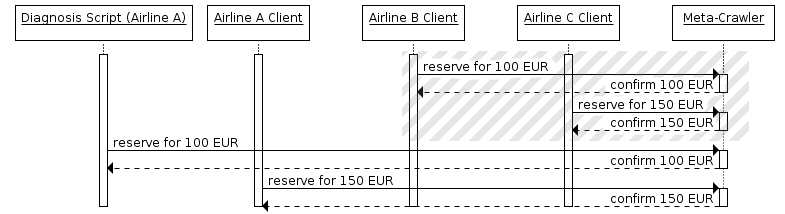
\includegraphics[width=\linewidth]{flyhehe-pass-pre-variation}
  \caption{Activity Prior To Successful Diagnosis}
  \label{fig:flyhehe-pre-booking}
\end{figure}

\subsection{Associating Variations and Assertions}
\label{sec:assoc-vari-with}

The diagnosis script is useful not only for producing similar
schedules, it also includes assertions that test the outcome of the
tested behavior. If the diagnosis reproduces a bug, those assertions
will fail.

Variances between passing and failing schedules can be used to reduce
the entry points that need to be checked for defects. If we compare
all passing schedules, we find variances that probably have no bearing
on the outcome of the test. If we compare them against the failing
schedules, and subtract the variances within the passes themselves, we
may find sequences that vary only between the passing and the failing
schedules. Those may be of particular interest to the developer,
because they are likely to be related to the failure. Such a variance
can occur in the unshaded activity in
\autoref{fig:flyhehe-pre-booking}. If the second reservation for
Airline A were sent prior to the receipt of the confirmation in the
diagnosis script, a critical race may ensue that causes the diagnosis
to fail.

Failing schedules have variances within themselves. We use this to
heuristically mark these variances as less likely causes than others,
as these variances then seem to have no impact on the outcome, since
they all produce the failure. Variances within the failure schedules
that also vary against all of the passing schedules are more likely to
be only on the path of the infected state of the program, not the
cause of the defect itself.

Consider \autoref{fig:flyhehe-failing-variation}, as an example for
variances in failing schedules. The failures, as the passes, may vary
in the order of reservations prior to the actual diagnosed
reservation---the shaded area near the top. However, the failures may
vary also in the order of the requests and confirmations for
reservations made by the diagnosis and the Airline A client---the
crossed area below. The only passing schedule for that part of the
communication is the one we see in
\autoref{fig:flyhehe-pre-booking}. Thus, the initial variances within
the failing schedule that also occur in the passes are of little
interest to the developer and need not be considered. The variances
near the end of the schedule, however, that are only between failing
schedules and do not vary within the passes can be considered likely
causes for the failure. We need to guide developers towards that part
of the communication for further debugging.

\begin{figure}
  \centering
  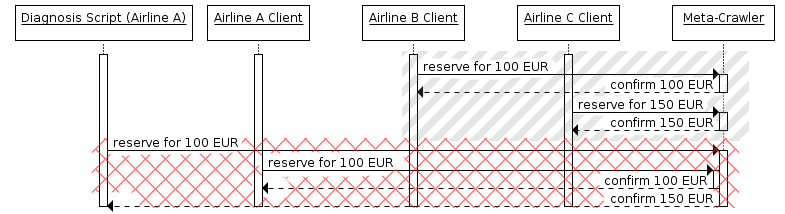
\includegraphics[width=\linewidth]{flyhehe-pass-failing-variation}
  \caption{Variations Failing Diagnosis Runs}
  \label{fig:flyhehe-failing-variation}
\end{figure}

% We could consider the interesting regions to be critical regions in
% the communication schedule, where even slight variations may cause a
% failure, and the variations that occur within passes as well can be
% considered forgiving regions of communication, where variance has
% little or no impact on the successful execution.

Finally events that occur late in the schedule are less likely to be
the original cause of a failure. To express this in our heuristic, we
adjust the probabilities linearly with respect to the sequence number
of the event within the schedule.

\section{Replay and Reordering}
\label{sec:comm-repl-reord}

Up to this point we have been inspecting the system without knowing
whether varying communication schedules are the cause for a
non-deterministic failure. We can now reinforce this assumption by
running failing schedules multiple times through what we call our
\emph{re-ordering replay scheduler}. The scheduler enforces a
particular order in network communication traces, which means we can
replay a failing trace multiple times with exactly the same order of
network events. If the result is consistently the same, even if the
failure occurred only sporadically before, we have a strong case to
believe that it was caused by this particular schedule, and further
inquiry with our method is warranted.

In some cases the outcome may vary even if our scheduler enforces a
failure schedule. An example is an improper implementation of
timestamp parsing on one machine, that causes the bug whenever the
timestamp has one of a few particular value. Such a bug will occur
regardless of the network schedule, and our approach is not suitable
to debug these kinds of failures. However, even in that case the
developer will have learned that non-determinism in the network
schedules is not responsible for the failure, and can focus his
debugging efforts on each server in turn, using traditional debugging
approaches.

\subsection{Re-ordering Scheduler}
\label{sec:re-order-sched}

The scheduler itself works as an intermediate layer between the
application code and the network, and effectively acts as a traffic
shaper\footnote{Internet standard definition of ``Shaper'' in RFC
  2475\\
  \url{http://tools.ietf.org/html/rfc2475\#section-2.3.3.3}\\
  accessed July 25, 2012}. It tries to re-order access to the shared
resource---the network---to enforce a particular, prerecorded
schedule. This is done by holding and releasing incoming and outgoing
communication according to the schedule, rather than the order in
which they arrive.

Since we want to record application layer events, it is most natural
to insert the scheduler between the application framework code
responsible for sending and receiving, and the underlying language or
operating system primitives. This has the additional advantage that
the scheduler can be programmed with some knowledge about the
framework, and thus the ability to communicate its actions to the
developer on the level of abstraction of the framework. This not only
keeps the developer in control of the debugging process, it also
allows meaningful configuration of the scheduler heuristics. Because
we record only the partial order and identifiers for communication
partners for events, the scheduler can only replay scheduled events
that occur in the system at the time of re-scheduling. That means that
\emph{all} servers that were active during record must be active
during replay as well. This may not always be the case, and scheduling
on the application layer allows us to communicate conditions for
holding and releasing events to the developers, so they can take
appropriate action, such as choosing another schedule or ensuring the
required servers are indeed online.

As an example, the scheduler can to re-order according to a schedule
that includes communication with a backup server. This backup server
may only be active at particular times of the day, say, at
night. Developers debugging a problem during the day may cause the
scheduler to wait for a long time---up until the backup server is
active. The system will seem to hang. Being able to communicate to the
developers the reason for waiting helps them to understand the
possible cause of the failure, and either bring the backup server
online for the purposes of debugging, or choose a schedule recorded at
another time.

Generally, such a scheduler has to control all points in a given
framework where application layer requests are received and
released. A possible algorithm for such a scheduler is given in
\autoref{fig:reorder-sched}. Such a scheduler will have to distinguish
whether the framework is using multiple threads of execution or just
one.

For our assumption of determinism on each server to hold,
multi-threaded servers need to be synchronized on send and receive
events, by using some kind of synchronization mechanism such as, for
example, semaphores. When a request is received, the scheduler checks
whether all requests that are expected to arrive before this request
have been received. If they have, the requests can be released into
the framework. Otherwise, the current thread of execution has to be
suspended until all previously scheduled requests have been
received. Upon release of a request into the framework, all threads
waiting on this request can be released, too. Similarly, for sending
responses, the scheduler holds those responses until all previously
scheduled responses have been sent by the framework.

Single threaded servers as they are used, for example, for event
loops, cannot be stopped if a request arrives too early, as that would
prevent any other requests from being processed. In this case, the
scheduler will receive requests into a buffer, and keep receiving
until the currently scheduled requests arrives, which is then
returned. Once the server is ready to process the next request, it may
be released directly from the buffer, if it was previously received,
skipping the network access altogether. In single-threaded mode we can
ignore outgoing requests. Under the assumption that the server works
deterministically, it will send the responses in the correct order if
it receives all requests in the correct order.

\begin{figure}
  \centering
  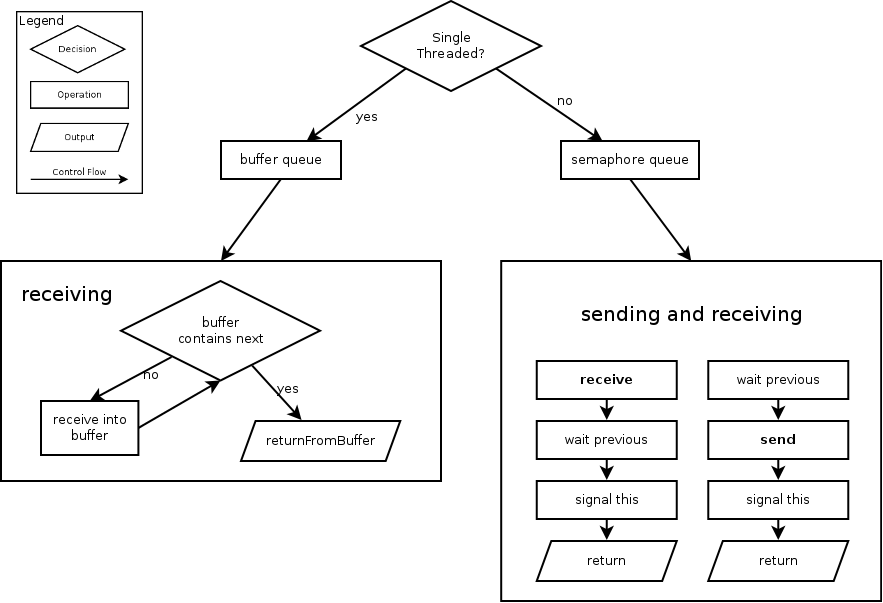
\includegraphics[width=\linewidth]{scheduler-ablaufdiagramm}
  \caption{FlowChart~\cite{Bohm1966} of Re-ordering Scheduler}
  \label{fig:reorder-sched}
\end{figure}

\subsection{Fault Navigation Over Multiple Runs}
\label{sec:replay-driven-fault}

After reproducing a failure, developers have to inspect the program
state. In \autoref{sec:lightweight-tracing} we have argued that a
lightweight logging approach is preferable for observations on the
live system, both to minimize the performance impact and the
possibility for Heisenbugs. However, this approach prohibits recording
information about the program state at this stage.

With the scheduler, however, we can enforce failure schedules as
needed for further analysis. Based on the initial communication log we
can, in a re-run, add an initial, shallow log of the called methods on
each node. This is based on the earlier work about incremental, online
analysis of runtime behavior~\cite{Perscheid2010}. Given the source
code running on the servers, this information can be connected in a
debugging tool to present a call tree to the developers.

While developers explore the call tree, it is interactively refined
on-demand. We add one-shot logging at points of interest as needed,
without disturbing the deployed system unduly. Because the the
scheduler holds on to parallel requests, the schedule will be
consistent with earlier runs and the program state will be a proper
sample.

\subsubsection{Recording the Right Data}
\label{sec:record-right-amount}

In order to assume that the observed program state for a particular
replay is a proper sample for this replay, we have to previously
record sufficient information to decide whether or not a given replay
is really equivalent to an earlier one. This means we may have to run
multiple replays for any given inquiry by the developer. Since we
record only the partial order and communication partners there is some
initial uncertainty about whether the message content is
equivalent.

Before any inquiry, we collect message samples for all communication
in a replay. This diminishes the aforementioned uncertainty, because,
on the application layer, we can treat message contents as parameters
to the remote system. This way, we can not only define a maximum
variance for messages to decide call equivalence, developers can also
review the message contents and decide, depending on the domain,
whether the schedule is correct.

\subsection{Online Replay}
\label{sec:online-replay}

In general our replay and record mechanism works for all the different
environments mentioned in \autoref{sec:observation-logging}, from
local developer setups to the deployed system. We consider the
deployed system to be the superior basis to acquire information during
replay.

A test environment already offers much better control to the
developers for debugging failures, even without the application of
Replay-driven Fault Navigation. Combined with our approach, we could
use the test environment to replace the diagnosis script with a more
"`traditional"' test, i.e a piece of executable code that resets the
test environment to a known state and then replays the recorded
live-system schedule within the test environment. Communication
partners that are part of the deployed, but not the test system have
to be mocked with prerecorded data.

The advantage of this way of using our approach is the amount of
control it offers. If the setup is sufficiently close to the deployed
system, the replay will inject the deployed system behavior into the
test environment. Multiple replays may be executed in quick
succession, as network and processing delays are small due to the
close physical proximity of servers in the test environment, and the
reduced load without live users that the system has to process, too.
Yet, those same variables may cause the test environment to produce
rare, non-deterministic failures at a different rate, or not at
all. Additionally, mocking servers that are not part of the test
environment introduces another uncertainty into the system, which
cannot be trivially proven to have no impact on the failure. Thus, we
focus on applying the replay mechanism directly to the deployed
systems.

\subsubsection{Distributed Recording}
\label{sec:distr-repl-reord}
\label{sec:distributed-scheduling}

Running debugger processes across a network and controlling them from
a developer machine introduces delays that prevent synchronous halt,
step, and resume. We circumvent these delays by using on-demand
scheduling and recording, yet, the question remains how to propagate
on-demand record in a synchronized manner in the distributed
system. We have not implemented such a mechanism, but different
designs come to mind, for the open-world case and the closed-world
case, respectively.

Our scheduler can be used to instrument some or all of the servers in
the deployed system, to replay schedules in the same environment in
which they were recorded. The advantage of this approach is the
availability of live data and more faithful reproduction of the
failure. It is non-trivial to reproduce the setup and state of a
sufficiently complex distributed system in a local test
environment. It may be easier to replay in the deployed system than to
re-create the deployment correctly enough to obtain the same execution
behavior.

In order to recover more data from the live system during replay than
we already have, the scheduler needs a mechanism specify recording
on-demand. This means that, while the developer is debugging, the
diagnosis script and scheduler replay the debugged schedule again and
again, each time recovering one more piece of information, like for
example a call stack, values of variables, and so on. Recovering only
one piece at a time means that developers have to wait until the
script has been re-executed and the information was recovered, but it
ensures minimal disruption to the service of the deployed system. This
impedes the fidelity of the approach outlined in approaches such as
the Path Tools~\cite{Perscheid2010}, which we build upon, but we show
that effective debugging is still possible with this approach
(\cf{\autoref{sec:wrapper-latency}}).

As mentioned above, our scheduler only works for well-behaved clients
in a functioning network, and in the absence of those, heuristics need
to be applied to ensure continued availability of the distributed
system overall. Since the scheduler cannot do more than wait for the
appropriate messages to appear to shape the traffic into the right
order, it depends entirely on network connectivity and deterministic
clients to reproduce a schedule. These constraints are not always met,
as network and server outages may make crucial parts of the schedule
temporarily unavailable. In this case, the scheduler will begin to
hold requests and responses on all nodes until temporary outage is
over. This is not desirable, as it effectively shuts the distributed
system down. We think that configurable heuristics for timeouts,
dropping requests or patterns for requests that should never be
rescheduled can circumvent this problem.

\paragraph{Closed-World Case}
\label{sec:clos-world-case}

In the closed-world case, all the servers in our distributed system
use our scheduler, and we have full control over the in- and output of
the system, both during record and replay. Also, no servers are added
or removed between record and replay.

During recording, each server generates a \ac{uuid} for itself, from
any suitable source such as the \textsc{mac} address of the network
card or the \ac{uuid} of other hardware components such as hard
disks. After the first execution, the log files from different servers
are aggregated into one and their \acp{uuid} are mapped to their
recorded \textsc{IP} addresses. Thus, the server \ac{uuid} allows us
to associate a server uniquely with events in the schedule.

During replay, the desired schedule is chosen at the developer
machine. The additionally desired information is added in form of
queries to the appropriate schedule event. For example, at the
beginning of a debugging session with a particular schedule, we
re-execute the schedule and for each event record the first few
hundred bytes of data sent or received. The schedule is split into
parts for each server that contributed to the original schedule and
sent out to those servers, via the same mechanism used to aggregate
the logs (\cf{\autoref{sec:mixed-environments}}). On each server the
scheduler will then read the log and re-order network access to suit
its partial schedule. Whenever an event with an additional query is
encountered, the scheduler will execute the query and log the result
before continuing its operations. At the end of each re-execution logs
are again aggregated from all participating servers and presented in
the debugger.

\paragraph{Open-World Case}
\label{sec:open-world-case}

In the open-world or mixed-world case, not all participating servers
include our scheduler or allow us to record at will---it may be
desirable, for example for Web services, to offer only replay data,
but not source code, to their developers. In the open-world case we
can also allow the number servers to change between record and replay.

In this case we record all message contents between scheduled and
non-scheduled servers. During the replay phase, any network event from
a non-scheduled to a scheduled server is performed with the recorded
data, not with the real network. The wrapped framework call for
network access is not executed. Likewise, any message sent to a
non-scheduled server during the record phase need not be sent again
during replay.

\subsubsection{Configuration Options}
\label{sec:required-heuristics}

For well-behaved clients in a closed-world setup the scheduler will be
able to perform its operation without problems, because given we start
with the right network event, all required events will eventually be
generated and the scheduler on each server can re-order events as
necessary. However, in the mixed-world case, with non-scheduled
servers, or in the face of unreliable network, with servers that
appear or disappear between record and replay---think of Web page
clients that use the deployed system while record and replay are in
progress---developers have to configure the scheduler to work under
these circumstances.

A scheduled server may receive events from servers that are not part
of the schedule, or wait to receive events from servers that were
available during record, but are not anymore during replay. We believe
this problem cannot be solved in a general way, and for these cases we
offer several settings with which developers can configure behavior
for these cases on each server.

\begin{description}
\item[Timeouts] Waiting for events may hold requests and responses
  unduly. A server that keeps no state between requests does not need
  to follow a schedule precisely for the re-execution to be
  useful. For example, in our flight reservation service, the Web page
  server has no state, as all the state is in the cache and airline
  databases. It may be useful to release network events after a
  configurable amount of time, regardless of their place in the
  schedule.
\item[Unscheduled Events] Non-scheduled servers may send events during
  replay that did not occur during record. If dropping these events is
  an option, it may be desirable to do so in order to keep the
  schedule. Otherwise, bypassing the schedule for these events may
  also work, depending on the setup---in our example clients that
  access the flight search during replay can bypass the schedule, as
  the search has no bearing on the reservation bug.
\item[Disruptions] It may be desirable to specify a separate timeout
  to wait for scheduled events. In our example the cache, which is
  queried for searches as well as rates and reservations, should not
  wait too long for an event. If a scheduled event is not generated in
  the network in time, the schedule should be marked as disrupted,
  re-scheduling is aborted, and all pending events are released. In
  this case the re-execution fails and has to be restarted.
\item[Message Level] Developers know their deployment setup best. If
  the re-execution is delayed, because the scheduler is waiting for a
  specific event to be generated from a specific server, this
  information may in itself be useful to the developers, even if the
  event never is generated. For example, if a backup is sent to
  another server from our flight cache every day at noon, and this
  caused a failure, replaying the schedule that includes the backup
  upload event can only work around noon, because otherwise the event
  is not generated. Informing the developer about this can be enough
  to provide a clue about the failure, and is preferable to stopping
  all network communication until the next backup network event is
  generated.
\end{description}

\section{Debugging at Different Levels of Granularity}
\label{sec:debugg-at-diff}

We can record and replay network schedules in the deployed system. We
use this mechanism to refining our recorded data during each
replay. The kind of additionally recorded data includes network event
contents, call stacks, method arguments, and return values. Developers
can use this information to associate events at the network
communication level to method activations at code level.

\subsection{Connecting Network Events to Code}
\label{sec:moving-from-network}

To debug asynchronously communicating applications developers need to
move between the different levels of abstraction, from communicating
servers to message sends between objects. They have to map the
observed network behavior to the original intentions expressed in the
code. In our approach we support this mapping with a tool that
integrates a network events with call trees.

One conventional approach to debugging distributed, communicating
applications is to try and determine likely locations of defects in
the code from the communication log, and the use a sequential debugger
to debug each server process independently to figure out which code
segment is responsible for a given unanticipated or erroneous network
event. However, with Web and other applications increasingly utilizing
asynchronous communication and event loops, mapping from code
locations to network events and back is becoming harder. While
outgoing requests can still be identified because they use only a
small number of framework calls for network communication, incoming
communication is increasingly handled by event callbacks. For this
style of communication, a debuggers' stack view will only reach back
as far as the last receive, with no possibility to look back further
to inspect previous communication events.

We propose tool support to provide an integrated view of both network
communication and call tree, synchronized to move freely from code to
network events and back. We argued that debugging across a network of
servers is similar to debugging across threads or communicating
objects. It appears natural to merge the communication trees and view
network communication as nested calls that originate from and return
to code. A debugging tool for distributed debugging may generally
support multiple, synchronized call trees, each call tree may show
network events or communicating objects.

Using our approach, developers are free to move through the recorded
execution both on the network level or on the code level. The
distributed debugger provides two synchronized views, one for the
global view on the network event log, and the other for a call tree
specific to the currently debugged server. Developers may interact
with the network view and, for example through clicking on an event, a
re-execution is triggered. This re-execution adds a query to the
schedule that logs all method activations on the server receiving the
event, in case of a request, or sending the event, in case of a
response. With that information, we can build an execution-specific
call tree for this server, and highlight the method activation that
was responsible for generating or receiving the network event. Since
we have recorded the full call tree, the developer is now free to move
up and down the call tree to orient himself in the code.

The debugging tool can use the information about sender and receiver
for each event to show the code that corresponds to the event. That
means showing the sender code for outgoing events and the receiver
code for incoming events. If the source code for a particular server
is available, the tool can automatically show the method responsible
for each communication event in the call tree. This provides
additional insight to the developers. They can then inspect method
arguments or local values, which will trigger additional re-executions
and recordings as needed, to find out more about how the event data is
generated or processed.

We have decided against adding support to show call trees from
multiple servers side by side, because we think the network event view
is more suitable to navigate from one server's call tree to
another. The interfaces between the different servers are encoded in
the communication data, rather than the arguments or local variables
in the servers' methods, so we think that presenting multiple call
trees side by side has no additional value.

\paragraph{Inferring Interfaces Across Languages}
\label{sec:inferr-interf-across}

A consequence of using our approach is the direct connection our
debugger can draw between code in different languages running on
different servers. Through the network events, we can infer interfaces
between those different languages. Those interfaces are implicitly
defined, in most \ac{rest} applications, or have more explicit
definitions only in another language, for example in \textsc{corba},
\textsc{soap}, or other kinds of middleware.

Without such explicit definitions so-called \ac{rest} interfaces
rarely follow a specific pattern for their communication. Oftentimes,
the wire encoding of choice is \ac{json}, because it is easy to use in
the browser and parser implementations exist for most
languages. However, \ac{json} as a simple key-value format for data
transfer offers no default interface definition language, and various
services\footnote{\xspace\hairspace
  Github API v3: \url{http://developer.github.com/v3/}\\
  Twitter REST API: \url{https://dev.twitter.com/docs/api}\\
  accessed July 25, 2012} offer no more than textual descriptions and
examples for their \ac{rest} \acp{api}. Such descriptions are hard to
verify against an implementation.

The more immediate issue with informal descriptions of \acp{api} is,
however, that outdated information is difficult to update, as this
requires checking the source code and update the documentation with
the informal \ac{api} description. With our approach, the interface
can be determined without access to the source code, by reviewing
recorded message contents for valid communication. If there is a
communication error somewhere in the log, and it is suspected to be
due to improper usage of the \ac{api}, the event's message contents
need only be compared against a log of a working communication, to
test this hypothesis.

Once such an error is discovered, our approach offers the direct
connection from the problematic events to the source code where the
events are generated and received. Thus, developers can test their
hypothesis and move to the appropriate piece of code to fix a
potential problem.

%%% Local Variables: 
%%% mode: latex
%%% TeX-master: "thesis"
%%% End: 

% \input{conclusions.tex}
% \chapter{Related Work}
\label{cha:related-work}

Because our approach combines work in various areas of distributed
systems debugging, from continuous record and replay, over
replay-driven fault navigation, debugging at different levels of
abstraction and full-on distributed debugging, we have sub-divided our
treaty of related work in this chapter into sections for each of those
domains.

\section{Record and Replay}
\label{sec:record-replay}

The need for consistent record and replay to debug certain kinds of
distributed applications is widely accepted. Approaches vary mainly in
how much they record, and subsequently how much of the system they can
simulate to eliminate behavioral disturbance.

\paragraph{Replay with Mocks}
\label{sec:replay-with-mocks}

Mocks are program entities designed to simulate the behavior of a real
entity. In system replay, mocks may be used to stand in for network
nodes. If enough information about the data sent by a particular node
has been recorded, there is no need to re-execute that node during
replay. Assuming the node works deterministically, a mock can return
the appropriate responses.

This approach is advantageous for nodes that are not under debugger
control. On those machines, package races on the network cannot be
rescheduled upon receive and behavior may still vary during
replay. Mocks avoid that problem, at the cost of greater recording
overhead at least in space, if not in time, for copying message
contents.

We have opted not to use mocks in this work, but other approaches use
mocks for some or all the nodes during a replay.

\paragraph{Deterministic Replay on the JVM with DejaVu}
\label{sec:dejavu}

\emph{DejaVu}~\cite{Konuru2000} is a record and replay framework for
distributed Java applications. It uses modified \acp{jvm} to execute
java applications and record their thread schedules as well as network
access. Thread and network schedules use implementations of Lamport
Clocks to establish event order.

The level of abstraction for network events in DejaVu is lower than in
this work, recording \ac{tcp} instead of \ac{http} events. While this
enables replay just as well, we argue that it is harder for a
programmer to review \ac{tcp} traffic and connect it to the program
domain than it is with \ac{http} events.

Contrary to this work, DejaVu supports both open and mixed world
record and replay. we note in \autoref{sec:distr-repl-reord} how the
same may be accomplished in my implementation.

\paragraph{Tracing and Simulation with iDNA}
\label{sec:idna}

\emph{iDNA}~\cite{Bhansali2006} is part of Microsoft-developed
framework for instruction-level tracing and replay of applications in
user-mode. The solution includes running instrumented programs atop a
runtime called \emph{Nirwana}, which provides hooks for iDNA to
register points of interest for tracing. The Nirwana runtime uses
dynamic binary translation to break a monitored process' instructions
into smaller instructions that are then instrumented and executed on
the host. The iDNA tracing component records traces via callbacks from
the Nirwana framework and, for replay, reads trace records and feeds
Nirwana desired instruction pointer and register values for
replay. The overhead is about one order of magnitude, which makes it
feasible to run IO-bound applications in tracing mode all the time,
which is also the scenario envisioned by the authors.

Due to its low level of recording, iDNA supports multi-threaded
applications, as well as applications that generate executable code at
runtime, such as \ac{jit}-compiled languages, but does not target networked
applications specifically. Similar to the present work, iDNA is aimed
at tracing continually on the live system, but the focus is on single
process applications rather than communicating processes or servers.

\paragraph{Reproducible Failures with ReCrash}
\label{sec:recrash}

\emph{ReCrash}~\cite{Artzi} is a framework to observe program execution in
Java and generate test-cases that reproduce observed errors. Similar
to this work, it can be applied to live systems. ReCrash does not try
to preserve enough information to replay an observed failure from the
beginning, but rather just keep enough information around to provide
an method entry point with arguments that trigger the crash.

To do this, ReCrash keeps a \emph{n}-deep \emph{shadow stack} during
execution with copies of the receivers and arguments. If a crash
occurs the stack is saved. In a second step, the shadow stack is
searched for the first call that reliably reproduces the exception.

The ability to reproduce crashes using this technique is limited by
the size of the shadow stack, as well as the copy depth of receiver
and arguments at each stage. Deeper stack and copying might be more
able to reproduce a crash, but imposes a larger overhead. The authors
offer a way out by only enabling monitoring after a crash occurred for
the first time, and only for methods on the stack at that point. Since
in this mode \emph{no} information has been saved about the execution,
the crash has to occur again, which might take a very long time for
rare exceptions.

For the class of problems that are related to causes that are not on
the same stack, like the concurrent update problem presented in this
thesis, ReCrash has only limited value.

\paragraph{Output-deterministic Replay with liblog}
\label{sec:liblog}

The \emph{liblog}~\cite{Geels2006Replay} tool for distributed C/C++
applications uses a {\tt libc} wrapper library to intercept system
calls and record events such as network communication, file access,
and \ac{ipc}.

The goal, as in this work, is to record sufficient information in the
live-system to replay execution at will for later debugging. The
authors decided against \emph{in-situ} replay, however, and use a
central console to download all logs and program checkpoints to
re-instantiate the program locally. Additionally, they record enough
information to replay each process independently of the others, which
imposes a higher tracing overhead.

Like DejaVu, and unlike this work, liblog records events at a very low
level. Most programs written for the Web, for example, do not use
socket programming directly, so the programmer will still have to
match the recorded network communication to the level of abstraction
in his code.

\section{Replay-driven Fault Navigation}
\label{sec:replay-driven-fault-1}

\paragraph{Test-driven Fault Navigation with Path Tools}
\label{sec:pathtools}

The \emph{Path Tools}~\cite{Perscheid} are a research project in
Squeak/Smalltalk and the basis for our prototype. Path Tools uses
re-executable entry points, mostly tests, to exercise code paths in a
project for analysis. These entry points need to execute
deterministically in order for the Path Tools' analysis to work
correctly.

In our work we have extended Path Tools and use it for re-execution
and analysis of distributed applications. Because Path Tools currently
need deterministic execution paths to work, this work offers an
approach to make network communication deterministic.

\section{Debugging at Different Levels of Abstraction}
\label{sec:debugg-at-diff-1}

\paragraph{Network Analysis and Debugging with Firebug}
\label{sec:firebug}

\emph{Firebug}\footnote{Mozilla Firebug:
  \url{http://getfirebug.com/}\\
  accessed June 20, 2012} is an open-source debugger and Web
application analysis tool for \emph{Firefox}\footnote{Mozilla Firefox:
  \url{http://www.mozilla.com/}\\
  accessed June 20, 2012}. It offers a JavaScript debugger with
breakpoints and a network pane to review \ac{xhr} requests made from
the JavaScript code of the web-page. Firebug includes the ability to
log network communication and set breakpoints on incoming and outgoing
connections, which enables developers to move from network to source
code, but not the other way around.

Firebug, like traditional debuggers, works synchronously on the code
and network communication of the current Web pages' JavaScript
process, and offers no integration with other services or debugger
instances. Also, while it is possible to break on network events and
move to the source code callback for a given event, there is no
further integration between the two~\cite{Barton2010}.

\paragraph{Message-oriented Debugging with Causeway}
\label{sec:causeway}

\emph{Causeway}\cite{Stanley2009} is a message-oriented debugger that
tries to unify the network request/response view with the message
send/receive view of the software. The authors' approach is to trace
program execution as well as network communication partners and
message contents, and present the captured information in a
post-mortem debugger. This debugger synchronizes the network and the
stack view so moving in one will update the other
(\cf{\autoref{fig:causeway}}), a behavior which has been the main
inspiration for how we show the two levels abstraction in our
prototype implementation.

In difference to this work, Causeway is strictly post-mortem. That
means it has to trace all required information, all the time, imposing
a very high overhead, a problem the authors mention themselves.

\begin{figure}[h]
  \centering
  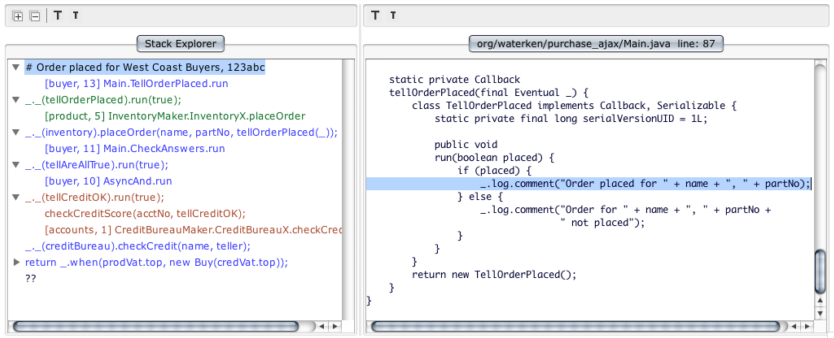
\includegraphics[width=0.7\linewidth]{causeway}
  \caption{Causeway Message Debugger}
  \label{fig:causeway}
\end{figure}

\section{Distributed Debugging}
\label{sec:distr-debugg}

Most debuggers work one thread at a time, and only for one process,
and offer the programmer a way to switch threads while debugging. Most
debuggers allow developers to stop all threads at once, however, this
disturb the execution order and lead to heisenbugs, since uniformly
starting and stopping multiple threads is not possible, even within a
single process. This equally applies to processes that are distributed
across a network. However, some runtimes, such as the \ac{jvm} or the
\ac{clr}, but also distributed systems middleware, such as
\textsc{corba}, still allow developers to stop and inspect processes
across a network.

\paragraph{Virtual Machine Interfaces on JVM and CLR}
\label{sec:java}

Both the \ac{jvm} and the \ac{clr} offer debugging facilities to
connect symbolic debuggers to remote processes. These facilities, in
case of the \ac{jvm} using a custom \ac{jvmti}\footnote{\textsc{jvm}
  Tool Interface Version 1.0\\
  \url{http://docs.oracle.com/javase/1.5.0/docs/guide/jvmti/jvmti.html}\\
  accessed July 31, 2012} and in case of the \ac{clr} built on the
\ac{com} standard~\cite{Strein2005}, abstract from the network to
offer the same debugging experience across a network as for local
processes. Debugging multiple processes from the same \ac{vm} is
possible with these approaches. Additionally, both of these \acp{vm}
are built to support different languages, so debugging across
languages is possible, too. However, we know of no debugging tool for
either \ac{vm} that supports different languages.

Compared to this work, these debugging interfaces have two
shortcomings: first, to inspect a remote process that process has to
be stopped by the debugger. It is undesirable for a deployed system to
stop providing its service because a debugger is connected to
it. Second, these debugging facilities only provide a view on the
program, and do not track network communication between processes, so
it is still difficult to get a global view of the distributed system.

\paragraph{Debugging Distributed Objects with CORBA and SOAP}
\label{sec:corba}

As a logical extension of object oriented programming into the realm
of distributed systems, middleware layers, such as
CORBA~\cite{Yang1996} and SOAP~\cite{Walsh2002}, have evolved. They
allow developers of distributed systems to specify object interfaces
for publishing and accessing distributed services in an
interchangeable format. Developers can program against these
interfaces as if the distributed system were running in a single
process, while the middleware takes care of communication. However,
much of the development time complexity hiding provided by middleware
is lost when debugging, because developers cannot step into message
sends that are converted to network communication by the
middleware. Recently, effort has been expended to enable symbolic
debuggers to overcome this restriction and step across
servers~\cite{Mega,Kaler2007} when debugging on top of such
middleware.

Such debuggers for middleware systems, like the middleware systems
themselves, try to abstract from the network. Approaches at stepping
across servers are extensions to symbolic debuggers that are meant to
allow developers to inspect objects in distributed system as if they
were locally available. In contrast to this work, these debuggers
target systems that are fully under developer control and can be
stopped at will for inspection. Like traditional symbolic debuggers,
they ignore Heisenbugs caused by the debugging process and are not
well suited to debug non-deterministic failures.

%%% Local Variables: 
%%% mode: latex
%%% TeX-master: "thesis"
%%% End: 


\bibliographystyle{model1-num-names}
\bibliography{paper}
\addcontentsline{toc}{section}{References}
\end{document}

%%% Local Variables: 
%%% mode: latex
%%% TeX-master: t
%%% End: 
